\documentclass[twoside]{book}

% Packages required by doxygen
\usepackage{calc}
\usepackage{doxygen}
\usepackage{graphicx}
\usepackage[utf8]{inputenc}
\usepackage{makeidx}
\usepackage{multicol}
\usepackage{multirow}
\usepackage{textcomp}
\usepackage[table]{xcolor}

% Font selection
\usepackage[T1]{fontenc}
\usepackage{mathptmx}
\usepackage[scaled=.90]{helvet}
\usepackage{courier}
\usepackage{amssymb}
\usepackage{sectsty}
\renewcommand{\familydefault}{\sfdefault}
\allsectionsfont{%
  \fontseries{bc}\selectfont%
  \color{darkgray}%
}
\renewcommand{\DoxyLabelFont}{%
  \fontseries{bc}\selectfont%
  \color{darkgray}%
}

% Page & text layout
\usepackage{geometry}
\geometry{%
  a4paper,%
  top=2.5cm,%
  bottom=2.5cm,%
  left=2.5cm,%
  right=2.5cm%
}
\tolerance=750
\hfuzz=15pt
\hbadness=750
\setlength{\emergencystretch}{15pt}
\setlength{\parindent}{0cm}
\setlength{\parskip}{0.2cm}
\makeatletter
\renewcommand{\paragraph}{%
  \@startsection{paragraph}{4}{0ex}{-1.0ex}{1.0ex}{%
    \normalfont\normalsize\bfseries\SS@parafont%
  }%
}
\renewcommand{\subparagraph}{%
  \@startsection{subparagraph}{5}{0ex}{-1.0ex}{1.0ex}{%
    \normalfont\normalsize\bfseries\SS@subparafont%
  }%
}
\makeatother

% Headers & footers
\usepackage{fancyhdr}
\pagestyle{fancyplain}
\fancyhead[LE]{\fancyplain{}{\bfseries\thepage}}
\fancyhead[CE]{\fancyplain{}{}}
\fancyhead[RE]{\fancyplain{}{\bfseries\leftmark}}
\fancyhead[LO]{\fancyplain{}{\bfseries\rightmark}}
\fancyhead[CO]{\fancyplain{}{}}
\fancyhead[RO]{\fancyplain{}{\bfseries\thepage}}
\fancyfoot[LE]{\fancyplain{}{}}
\fancyfoot[CE]{\fancyplain{}{}}
\fancyfoot[RE]{\fancyplain{}{\bfseries\scriptsize Generated on Wed May 14 2014 18\-:30\-:38 for Arbetsprov by Doxygen }}
\fancyfoot[LO]{\fancyplain{}{\bfseries\scriptsize Generated on Wed May 14 2014 18\-:30\-:38 for Arbetsprov by Doxygen }}
\fancyfoot[CO]{\fancyplain{}{}}
\fancyfoot[RO]{\fancyplain{}{}}
\renewcommand{\footrulewidth}{0.4pt}
\renewcommand{\chaptermark}[1]{%
  \markboth{#1}{}%
}
\renewcommand{\sectionmark}[1]{%
  \markright{\thesection\ #1}%
}

% Indices & bibliography
\usepackage{natbib}
\usepackage[titles]{tocloft}
\setcounter{tocdepth}{3}
\setcounter{secnumdepth}{5}
\makeindex

% Hyperlinks (required, but should be loaded last)
\usepackage{ifpdf}
\ifpdf
  \usepackage[pdftex,pagebackref=true]{hyperref}
\else
  \usepackage[ps2pdf,pagebackref=true]{hyperref}
\fi
\hypersetup{%
  colorlinks=true,%
  linkcolor=blue,%
  citecolor=blue,%
  unicode%
}

% Custom commands
\newcommand{\clearemptydoublepage}{%
  \newpage{\pagestyle{empty}\cleardoublepage}%
}


%===== C O N T E N T S =====

\begin{document}

% Titlepage & ToC
\hypersetup{pageanchor=false}
\pagenumbering{roman}
\begin{titlepage}
\vspace*{7cm}
\begin{center}%
{\Large Arbetsprov }\\
\vspace*{1cm}
{\large Generated by Doxygen 1.8.5}\\
\vspace*{0.5cm}
{\small Wed May 14 2014 18:30:38}\\
\end{center}
\end{titlepage}
\clearemptydoublepage
\tableofcontents
\clearemptydoublepage
\pagenumbering{arabic}
\hypersetup{pageanchor=true}

%--- Begin generated contents ---
\chapter{Namespace Index}
\section{Namespace List}
Here is a list of all documented namespaces with brief descriptions\-:\begin{DoxyCompactList}
\item\contentsline{section}{\hyperlink{namespacearbestprov}{arbestprov} }{\pageref{namespacearbestprov}}{}
\item\contentsline{section}{\hyperlink{namespacearbetsprov}{arbetsprov} }{\pageref{namespacearbetsprov}}{}
\end{DoxyCompactList}

\chapter{Hierarchical Index}
\section{Class Hierarchy}
This inheritance list is sorted roughly, but not completely, alphabetically\-:\begin{DoxyCompactList}
\item \contentsline{section}{abstract\-Controller}{\pageref{classabstract_controller}}{}
\begin{DoxyCompactList}
\item \contentsline{section}{controller\-Base}{\pageref{classcontroller_base}}{}
\begin{DoxyCompactList}
\item \contentsline{section}{index\-Controller}{\pageref{classindex_controller}}{}
\item \contentsline{section}{program\-Controller}{\pageref{classprogram_controller}}{}
\end{DoxyCompactList}
\end{DoxyCompactList}
\item Array\-Object\begin{DoxyCompactList}
\item \contentsline{section}{Registry}{\pageref{class_registry}}{}
\end{DoxyCompactList}
\item \contentsline{section}{Config}{\pageref{class_config}}{}
\item \contentsline{section}{db}{\pageref{classdb}}{}
\item \contentsline{section}{debug}{\pageref{classdebug}}{}
\item Iterator\-Aggregate\begin{DoxyCompactList}
\item \contentsline{section}{Array\-Object\-Wrapper}{\pageref{class_array_object_wrapper}}{}
\end{DoxyCompactList}
\item \contentsline{section}{Page\-Fragment\-Base}{\pageref{class_page_fragment_base}}{}
\begin{DoxyCompactList}
\item \contentsline{section}{program\-Display\-Block}{\pageref{classprogram_display_block}}{}
\end{DoxyCompactList}
\item \contentsline{section}{program}{\pageref{classprogram}}{}
\item \contentsline{section}{Router}{\pageref{class_router}}{}
\item \contentsline{section}{Template}{\pageref{class_template}}{}
\item \contentsline{section}{Util}{\pageref{class_util}}{}
\item \contentsline{section}{Xml\-Util}{\pageref{class_xml_util}}{}
\end{DoxyCompactList}

\chapter{Data Structure Index}
\section{Data Structures}
Here are the data structures with brief descriptions\-:\begin{DoxyCompactList}
\item\contentsline{section}{\hyperlink{classabstract_controller}{abstract\-Controller} }{\pageref{classabstract_controller}}{}
\item\contentsline{section}{\hyperlink{class_array_object_wrapper}{Array\-Object\-Wrapper} }{\pageref{class_array_object_wrapper}}{}
\item\contentsline{section}{\hyperlink{class_config}{Config} }{\pageref{class_config}}{}
\item\contentsline{section}{\hyperlink{classcontroller_base}{controller\-Base} }{\pageref{classcontroller_base}}{}
\item\contentsline{section}{\hyperlink{classdb}{db} }{\pageref{classdb}}{}
\item\contentsline{section}{\hyperlink{classdebug}{debug} }{\pageref{classdebug}}{}
\item\contentsline{section}{\hyperlink{classindex_controller}{index\-Controller} }{\pageref{classindex_controller}}{}
\item\contentsline{section}{\hyperlink{class_page_fragment_base}{Page\-Fragment\-Base} }{\pageref{class_page_fragment_base}}{}
\item\contentsline{section}{\hyperlink{classprogram}{program} }{\pageref{classprogram}}{}
\item\contentsline{section}{\hyperlink{classprogram_controller}{program\-Controller} }{\pageref{classprogram_controller}}{}
\item\contentsline{section}{\hyperlink{classprogram_display_block}{program\-Display\-Block} }{\pageref{classprogram_display_block}}{}
\item\contentsline{section}{\hyperlink{class_registry}{Registry} }{\pageref{class_registry}}{}
\item\contentsline{section}{\hyperlink{class_router}{Router} }{\pageref{class_router}}{}
\item\contentsline{section}{\hyperlink{class_template}{Template} }{\pageref{class_template}}{}
\item\contentsline{section}{\hyperlink{class_util}{Util} }{\pageref{class_util}}{}
\item\contentsline{section}{\hyperlink{class_xml_util}{Xml\-Util} }{\pageref{class_xml_util}}{}
\end{DoxyCompactList}

\chapter{Namespace Documentation}
\hypertarget{namespacearbestprov}{\section{arbestprov Namespace Reference}
\label{namespacearbestprov}\index{arbestprov@{arbestprov}}
}


\subsection{Detailed Description}
View script for a H\-T\-M\-L page footer

\begin{DoxySince}{Since}
Aug 2010 \-::views 
\end{DoxySince}

\hypertarget{namespacearbetsprov}{\section{arbetsprov Namespace Reference}
\label{namespacearbetsprov}\index{arbetsprov@{arbetsprov}}
}


\subsection{Detailed Description}
Autoprependfile -\/ contains the lowlevel stuff

\begin{DoxyAuthor}{Author}
P\-A Ulander, \href{mailto:pa@kabelkultur.se}{\tt pa@kabelkultur.\-se} 
\end{DoxyAuthor}
\begin{DoxySince}{Since}
August 2010
\end{DoxySince}
Baseclass for all controllers and requests

\begin{DoxyAuthor}{Author}
P\-A Ulander, \href{mailto:pa@kabelkultur.se}{\tt pa@kabelkultur.\-se} 
\end{DoxyAuthor}
\begin{DoxySince}{Since}
Aug 2010
\end{DoxySince}
require base controller Base class for all controller actions

\begin{DoxyAuthor}{Author}
P\-A Ulander, \href{mailto:pa@kabelkultur.se}{\tt pa@kabelkultur.\-se} 
\end{DoxyAuthor}
\begin{DoxySince}{Since}
Aug 2010
\end{DoxySince}
Controller class for all common pages

\begin{DoxyAuthor}{Author}
P\-A Ulander \href{mailto:pa@kabelkultur.se}{\tt pa@kabelkultur.\-se} 
\end{DoxyAuthor}
\begin{DoxySince}{Since}
Aug 2010
\end{DoxySince}
Controller class for programs

\begin{DoxyAuthor}{Author}
P\-A Ulander \href{mailto:pa@kabelkultur.se}{\tt pa@kabelkultur.\-se} 
\end{DoxyAuthor}
\begin{DoxySince}{Since}
Aug 2010
\end{DoxySince}
Simple connection wrapper for using with P\-D\-O

\begin{DoxyAuthor}{Author}
P\-A Ulander, \href{mailto:pa@kabelkultur.se}{\tt pa@kabelkultur.\-se} 
\end{DoxyAuthor}
\begin{DoxySince}{Since}
Aug 2010
\end{DoxySince}
Array\-Object wrapper to allow for paralel array maps in memory

\begin{DoxyAuthor}{Author}
P\-A Ulander, \href{mailto:pa@kabelkultur.se}{\tt pa@kabelkultur.\-se} 
\end{DoxyAuthor}
\begin{DoxySince}{Since}
Nov 2010
\end{DoxySince}
Class used to initiate the application configuration object

\begin{DoxyAuthor}{Author}
P\-A Ulander, \href{mailto:pa@kabelkultur.se}{\tt pa@kabelkultur.\-se} 
\end{DoxyAuthor}
\begin{DoxySince}{Since}
Aug 2010
\end{DoxySince}
Class used to initiate a registry object

\begin{DoxyAuthor}{Author}
P\-A Ulander, \href{mailto:pa@kabelkultur.se}{\tt pa@kabelkultur.\-se} 
\end{DoxyAuthor}
\begin{DoxySince}{Since}
Aug 2010
\end{DoxySince}
Simple not so fancy router class

\begin{DoxyAuthor}{Author}
P\-A Ulander, \href{mailto:pa@kabelkultur.se}{\tt pa@kabelkultur.\-se} 
\end{DoxyAuthor}
\begin{DoxySince}{Since}
Aug 2010
\end{DoxySince}
Templating base class

\begin{DoxyAuthor}{Author}
P\-A Ulander, \href{mailto:pa@kabelkultur.se}{\tt pa@kabelkultur.\-se} 
\end{DoxyAuthor}
\begin{DoxySince}{Since}
Aug 2010
\end{DoxySince}
Databean like class representing a row of program data

\begin{DoxyAuthor}{Author}
P\-A Ulander, \href{mailto:pa@kabelkultur.se}{\tt pa@kabelkultur.\-se} 
\end{DoxyAuthor}
\begin{DoxySince}{Since}
Aug 2010
\end{DoxySince}
Class that represents the data to display

\begin{DoxyAuthor}{Author}
P\-A Ulander, \href{mailto:pa@kabelkultur.se}{\tt pa@kabelkultur.\-se} 
\end{DoxyAuthor}
\begin{DoxySince}{Since}
Aug 2010
\end{DoxySince}
Base class for page fragment classes

\begin{DoxyAuthor}{Author}
P\-A Ulander, \href{mailto:pa@kabelkultur.se}{\tt pa@kabelkultur.\-se} 
\end{DoxyAuthor}
\begin{DoxySince}{Since}
Aug 2010
\end{DoxySince}
Class containing some utility like methods

\begin{DoxyAuthor}{Author}
P\-A Ulander, \href{mailto:pa@kabelkultur.se}{\tt pa@kabelkultur.\-se} 
\end{DoxyAuthor}
\begin{DoxySince}{Since}
Aug 2010
\end{DoxySince}
View script for a head section of a H\-T\-M\-L page

\begin{DoxySince}{Since}
Aug 2010 \-::views
\end{DoxySince}
View script for a H\-T\-M\-L pagebody

\begin{DoxySince}{Since}
Aug 2010 \-::views
\end{DoxySince}
View script for a H\-T\-M\-L page footer

\begin{DoxySince}{Since}
Aug 2010 \-::views
\end{DoxySince}
A simple class for dealing with xml

\begin{DoxyAuthor}{Author}
P\-A Ulander, \href{mailto:pa@kabelkultur.se}{\tt pa@kabelkultur.\-se} 
\end{DoxyAuthor}
\begin{DoxySince}{Since}
Aug 2010 
\end{DoxySince}

\chapter{Data Structure Documentation}
\hypertarget{classabstract_controller}{\section{abstract\-Controller Class Reference}
\label{classabstract_controller}\index{abstract\-Controller@{abstract\-Controller}}
}
Inheritance diagram for abstract\-Controller\-:\begin{figure}[H]
\begin{center}
\leavevmode
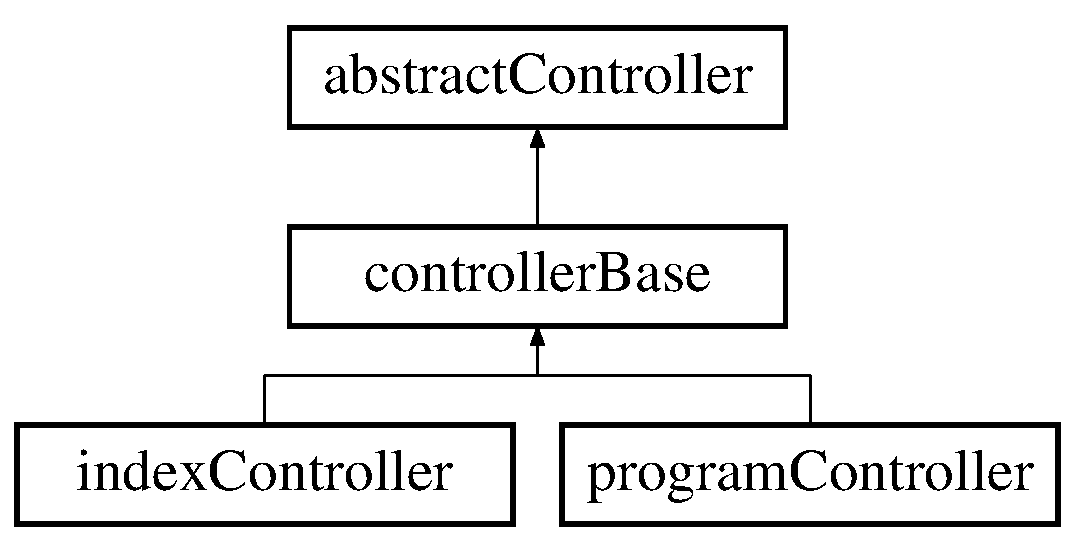
\includegraphics[height=3.000000cm]{classabstract_controller}
\end{center}
\end{figure}
\subsection*{Public Member Functions}
\begin{DoxyCompactItemize}
\item 
\hyperlink{classabstract_controller_a095c5d389db211932136b53f25f39685}{\-\_\-\-\_\-construct} ()
\item 
\hyperlink{classabstract_controller_a4be4055f3361d4800e16bc2e2e38cda6}{init} ()
\item 
\hyperlink{classabstract_controller_adf1a35ad20e475c59cc0967d5764aa22}{get\-Request} ()
\item 
\hyperlink{classabstract_controller_a346a92c94dc686c7217f35a078b5a54f}{set\-Request} (\$p\-\_\-s\-Request)
\end{DoxyCompactItemize}
\subsection*{Protected Attributes}
\begin{DoxyCompactItemize}
\item 
\hypertarget{classabstract_controller_a815262d9bd8ab6e610f85e2b45bb13ec}{{\bfseries \$s\-Request} = null}\label{classabstract_controller_a815262d9bd8ab6e610f85e2b45bb13ec}

\end{DoxyCompactItemize}


\subsection{Constructor \& Destructor Documentation}
\hypertarget{classabstract_controller_a095c5d389db211932136b53f25f39685}{\index{abstract\-Controller@{abstract\-Controller}!\-\_\-\-\_\-construct@{\-\_\-\-\_\-construct}}
\index{\-\_\-\-\_\-construct@{\-\_\-\-\_\-construct}!abstractController@{abstract\-Controller}}
\subsubsection[{\-\_\-\-\_\-construct}]{\setlength{\rightskip}{0pt plus 5cm}\-\_\-\-\_\-construct (
\begin{DoxyParamCaption}
{}
\end{DoxyParamCaption}
)}}\label{classabstract_controller_a095c5d389db211932136b53f25f39685}
Constructor for this instance 

\subsection{Member Function Documentation}
\hypertarget{classabstract_controller_adf1a35ad20e475c59cc0967d5764aa22}{\index{abstract\-Controller@{abstract\-Controller}!get\-Request@{get\-Request}}
\index{get\-Request@{get\-Request}!abstractController@{abstract\-Controller}}
\subsubsection[{get\-Request}]{\setlength{\rightskip}{0pt plus 5cm}get\-Request (
\begin{DoxyParamCaption}
{}
\end{DoxyParamCaption}
)}}\label{classabstract_controller_adf1a35ad20e475c59cc0967d5764aa22}
Getter for Request

\begin{DoxyReturn}{Returns}
string 
\end{DoxyReturn}
\hypertarget{classabstract_controller_a4be4055f3361d4800e16bc2e2e38cda6}{\index{abstract\-Controller@{abstract\-Controller}!init@{init}}
\index{init@{init}!abstractController@{abstract\-Controller}}
\subsubsection[{init}]{\setlength{\rightskip}{0pt plus 5cm}init (
\begin{DoxyParamCaption}
{}
\end{DoxyParamCaption}
)}}\label{classabstract_controller_a4be4055f3361d4800e16bc2e2e38cda6}
Initialize object

Called from \hyperlink{classabstract_controller_a095c5d389db211932136b53f25f39685}{\-\_\-\-\_\-construct()} as final step of object instantiation.

\begin{DoxyReturn}{Returns}
void 
\end{DoxyReturn}
\hypertarget{classabstract_controller_a346a92c94dc686c7217f35a078b5a54f}{\index{abstract\-Controller@{abstract\-Controller}!set\-Request@{set\-Request}}
\index{set\-Request@{set\-Request}!abstractController@{abstract\-Controller}}
\subsubsection[{set\-Request}]{\setlength{\rightskip}{0pt plus 5cm}set\-Request (
\begin{DoxyParamCaption}
\item[{}]{\$p\-\_\-s\-Request}
\end{DoxyParamCaption}
)}}\label{classabstract_controller_a346a92c94dc686c7217f35a078b5a54f}
Setter for Request


\begin{DoxyParams}[1]{Parameters}
string\-\_\-type & {\em \$p\-\_\-s\-Request} & \\
\hline
\end{DoxyParams}


The documentation for this class was generated from the following file\-:\begin{DoxyCompactItemize}
\item 
/home/pa/web-\/projects/arbetsprov-\/project/arbetsprov.\-git/arbetsprov/application/controllers/abstract\-Controller.\-php\end{DoxyCompactItemize}

\hypertarget{class_array_object_wrapper}{\section{Array\-Object\-Wrapper Class Reference}
\label{class_array_object_wrapper}\index{Array\-Object\-Wrapper@{Array\-Object\-Wrapper}}
}
Inheritance diagram for Array\-Object\-Wrapper\-:\begin{figure}[H]
\begin{center}
\leavevmode
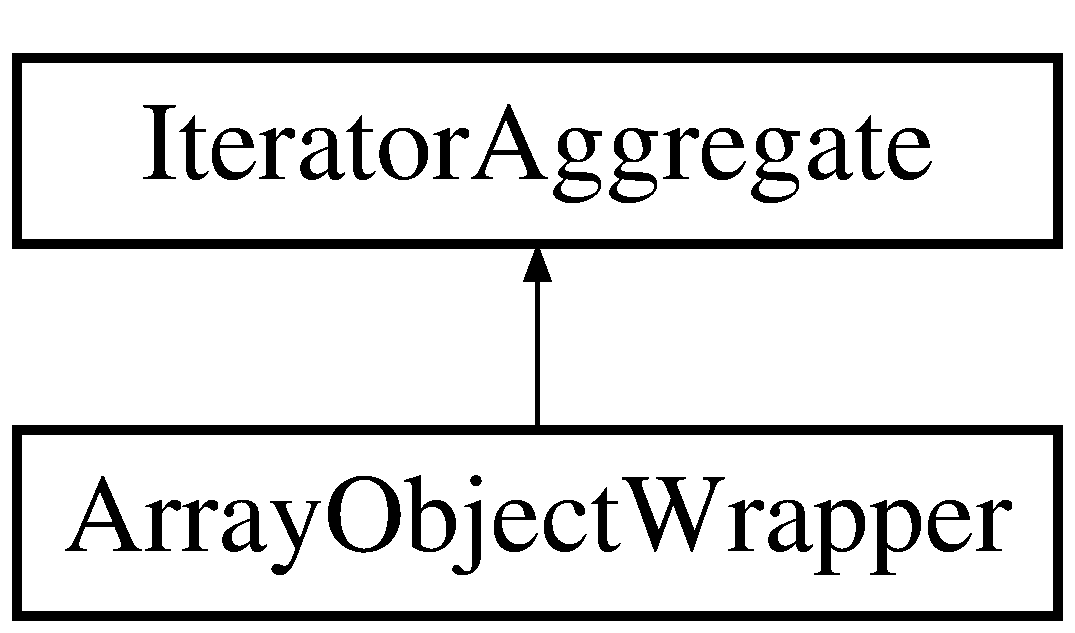
\includegraphics[height=2.000000cm]{class_array_object_wrapper}
\end{center}
\end{figure}
\subsection*{Public Member Functions}
\begin{DoxyCompactItemize}
\item 
\hyperlink{class_array_object_wrapper_a669fafc99ae523832111df9ff419c26f}{\-\_\-\-\_\-construct} (\$p\-\_\-a\-Array=array(), \$p\-\_\-i\-Flags=null)
\item 
\hyperlink{class_array_object_wrapper_a5b929cc9927db3604334c4440ec000a4}{append} (\$p\-\_\-m\-Object\-To\-Append)
\item 
\hyperlink{class_array_object_wrapper_ac751e87b3d4c4bf2feb03bee8b092755}{count} ()
\item 
\hyperlink{class_array_object_wrapper_a7a9f937c2958e6f4dd7b030f86fb70b7}{get\-Iterator} ()
\item 
\hyperlink{class_array_object_wrapper_a0d140ee670ddd77874232f083bef932d}{offset\-Exists} (\$p\-\_\-m\-Index)
\item 
\hyperlink{class_array_object_wrapper_aa160b823e136d400f9ffd480f25b5f71}{offset\-Get} (\$p\-\_\-m\-Index)
\item 
\hyperlink{class_array_object_wrapper_a4930cef3acef8460f7f0517791f188b1}{offset\-Set} (\$p\-\_\-m\-Index, \$p\-\_\-m\-Value)
\item 
\hyperlink{class_array_object_wrapper_a030879cbf382538eb70f3a2db8a0a15c}{offset\-Unset} (\$p\-\_\-m\-Index)
\end{DoxyCompactItemize}


\subsection{Constructor \& Destructor Documentation}
\hypertarget{class_array_object_wrapper_a669fafc99ae523832111df9ff419c26f}{\index{Array\-Object\-Wrapper@{Array\-Object\-Wrapper}!\-\_\-\-\_\-construct@{\-\_\-\-\_\-construct}}
\index{\-\_\-\-\_\-construct@{\-\_\-\-\_\-construct}!ArrayObjectWrapper@{Array\-Object\-Wrapper}}
\subsubsection[{\-\_\-\-\_\-construct}]{\setlength{\rightskip}{0pt plus 5cm}\-\_\-\-\_\-construct (
\begin{DoxyParamCaption}
\item[{}]{\$p\-\_\-a\-Array = {\ttfamily array()}, }
\item[{}]{\$p\-\_\-i\-Flags = {\ttfamily null}}
\end{DoxyParamCaption}
)}}\label{class_array_object_wrapper_a669fafc99ae523832111df9ff419c26f}
Constructor which instantiates \$this-\/$>$o\-Container


\begin{DoxyParams}[1]{Parameters}
array & {\em \$p\-\_\-a\-Array} & Optional \\
\hline
int & {\em \$p\-\_\-i\-Flags} & Optional \\
\hline
\end{DoxyParams}


\subsection{Member Function Documentation}
\hypertarget{class_array_object_wrapper_a5b929cc9927db3604334c4440ec000a4}{\index{Array\-Object\-Wrapper@{Array\-Object\-Wrapper}!append@{append}}
\index{append@{append}!ArrayObjectWrapper@{Array\-Object\-Wrapper}}
\subsubsection[{append}]{\setlength{\rightskip}{0pt plus 5cm}append (
\begin{DoxyParamCaption}
\item[{}]{\$p\-\_\-m\-Object\-To\-Append}
\end{DoxyParamCaption}
)}}\label{class_array_object_wrapper_a5b929cc9927db3604334c4440ec000a4}
Does an \hyperlink{class_array_object_wrapper_a5b929cc9927db3604334c4440ec000a4}{append()} call on the wrapped Array\-Object instance


\begin{DoxyParams}[1]{Parameters}
mixed & {\em \$p\-\_\-m\-Object\-To\-Append} & \\
\hline
\end{DoxyParams}
\hypertarget{class_array_object_wrapper_ac751e87b3d4c4bf2feb03bee8b092755}{\index{Array\-Object\-Wrapper@{Array\-Object\-Wrapper}!count@{count}}
\index{count@{count}!ArrayObjectWrapper@{Array\-Object\-Wrapper}}
\subsubsection[{count}]{\setlength{\rightskip}{0pt plus 5cm}count (
\begin{DoxyParamCaption}
{}
\end{DoxyParamCaption}
)}}\label{class_array_object_wrapper_ac751e87b3d4c4bf2feb03bee8b092755}
Does a \hyperlink{class_array_object_wrapper_ac751e87b3d4c4bf2feb03bee8b092755}{count()} call on the wrapped Array\-Object instance

\begin{DoxyReturn}{Returns}
int Number of elements in \$this-\/$>$o\-Container 
\end{DoxyReturn}
\hypertarget{class_array_object_wrapper_a7a9f937c2958e6f4dd7b030f86fb70b7}{\index{Array\-Object\-Wrapper@{Array\-Object\-Wrapper}!get\-Iterator@{get\-Iterator}}
\index{get\-Iterator@{get\-Iterator}!ArrayObjectWrapper@{Array\-Object\-Wrapper}}
\subsubsection[{get\-Iterator}]{\setlength{\rightskip}{0pt plus 5cm}get\-Iterator (
\begin{DoxyParamCaption}
{}
\end{DoxyParamCaption}
)}}\label{class_array_object_wrapper_a7a9f937c2958e6f4dd7b030f86fb70b7}
Does a \hyperlink{class_array_object_wrapper_a7a9f937c2958e6f4dd7b030f86fb70b7}{get\-Iterator()} call on the wrapped Array\-Object instance

\begin{DoxyReturn}{Returns}
Array\-Iterator The iterator of \$this-\/$>$o\-Container 
\end{DoxyReturn}
\hypertarget{class_array_object_wrapper_a0d140ee670ddd77874232f083bef932d}{\index{Array\-Object\-Wrapper@{Array\-Object\-Wrapper}!offset\-Exists@{offset\-Exists}}
\index{offset\-Exists@{offset\-Exists}!ArrayObjectWrapper@{Array\-Object\-Wrapper}}
\subsubsection[{offset\-Exists}]{\setlength{\rightskip}{0pt plus 5cm}offset\-Exists (
\begin{DoxyParamCaption}
\item[{}]{\$p\-\_\-m\-Index}
\end{DoxyParamCaption}
)}}\label{class_array_object_wrapper_a0d140ee670ddd77874232f083bef932d}
Does an \hyperlink{class_array_object_wrapper_a0d140ee670ddd77874232f083bef932d}{offset\-Exists()} call on the wrapped Array\-Object instance


\begin{DoxyParams}[1]{Parameters}
mixed & {\em \$p\-\_\-m\-Index} & \\
\hline
 & {\em bool} & True if \$p\-\_\-m\-Index is set, otherwise false \\
\hline
\end{DoxyParams}
\hypertarget{class_array_object_wrapper_aa160b823e136d400f9ffd480f25b5f71}{\index{Array\-Object\-Wrapper@{Array\-Object\-Wrapper}!offset\-Get@{offset\-Get}}
\index{offset\-Get@{offset\-Get}!ArrayObjectWrapper@{Array\-Object\-Wrapper}}
\subsubsection[{offset\-Get}]{\setlength{\rightskip}{0pt plus 5cm}offset\-Get (
\begin{DoxyParamCaption}
\item[{}]{\$p\-\_\-m\-Index}
\end{DoxyParamCaption}
)}}\label{class_array_object_wrapper_aa160b823e136d400f9ffd480f25b5f71}
Does an \hyperlink{class_array_object_wrapper_aa160b823e136d400f9ffd480f25b5f71}{offset\-Get()} call on the wrapped Array\-Object instance


\begin{DoxyParams}[1]{Parameters}
mixed & {\em \$p\-\_\-m\-Index} & \\
\hline
\end{DoxyParams}
\begin{DoxyReturn}{Returns}
mixed Stored object (variable) having index \$p\-\_\-m\-Index 
\end{DoxyReturn}
\hypertarget{class_array_object_wrapper_a4930cef3acef8460f7f0517791f188b1}{\index{Array\-Object\-Wrapper@{Array\-Object\-Wrapper}!offset\-Set@{offset\-Set}}
\index{offset\-Set@{offset\-Set}!ArrayObjectWrapper@{Array\-Object\-Wrapper}}
\subsubsection[{offset\-Set}]{\setlength{\rightskip}{0pt plus 5cm}offset\-Set (
\begin{DoxyParamCaption}
\item[{}]{\$p\-\_\-m\-Index, }
\item[{}]{\$p\-\_\-m\-Value}
\end{DoxyParamCaption}
)}}\label{class_array_object_wrapper_a4930cef3acef8460f7f0517791f188b1}
Does an \hyperlink{class_array_object_wrapper_a4930cef3acef8460f7f0517791f188b1}{offset\-Set()} call on the wrapped Array\-Object instance


\begin{DoxyParams}[1]{Parameters}
mixed & {\em \$p\-\_\-m\-Index} & \\
\hline
mixed & {\em \$p\-\_\-m\-Value} & \\
\hline
\end{DoxyParams}
\hypertarget{class_array_object_wrapper_a030879cbf382538eb70f3a2db8a0a15c}{\index{Array\-Object\-Wrapper@{Array\-Object\-Wrapper}!offset\-Unset@{offset\-Unset}}
\index{offset\-Unset@{offset\-Unset}!ArrayObjectWrapper@{Array\-Object\-Wrapper}}
\subsubsection[{offset\-Unset}]{\setlength{\rightskip}{0pt plus 5cm}offset\-Unset (
\begin{DoxyParamCaption}
\item[{}]{\$p\-\_\-m\-Index}
\end{DoxyParamCaption}
)}}\label{class_array_object_wrapper_a030879cbf382538eb70f3a2db8a0a15c}
Does an \hyperlink{class_array_object_wrapper_a030879cbf382538eb70f3a2db8a0a15c}{offset\-Unset()} call on the wrapped Array\-Object instance


\begin{DoxyParams}[1]{Parameters}
mixed & {\em \$p\-\_\-m\-Index} & \\
\hline
\end{DoxyParams}


The documentation for this class was generated from the following file\-:\begin{DoxyCompactItemize}
\item 
/home/pa/web-\/projects/arbetsprov-\/project/arbetsprov.\-git/arbetsprov/application/lib/Array\-Object\-Wrapper.\-php\end{DoxyCompactItemize}

\hypertarget{class_config}{\section{Config Class Reference}
\label{class_config}\index{Config@{Config}}
}
\subsection*{Public Member Functions}
\begin{DoxyCompactItemize}
\item 
\hyperlink{class_config_a4aec4f4555fcea8f52c10a967d17434c}{\-\_\-\-\_\-get} (\$p\-\_\-s\-Config\-Key)
\end{DoxyCompactItemize}
\subsection*{Static Public Member Functions}
\begin{DoxyCompactItemize}
\item 
static \hyperlink{class_config_a9c67b75c16c239bb556c093b4145e235}{get\-Instance} (\$p\-\_\-s\-Ini\-File\-Path)
\end{DoxyCompactItemize}


\subsection{Member Function Documentation}
\hypertarget{class_config_a4aec4f4555fcea8f52c10a967d17434c}{\index{Config@{Config}!\-\_\-\-\_\-get@{\-\_\-\-\_\-get}}
\index{\-\_\-\-\_\-get@{\-\_\-\-\_\-get}!Config@{Config}}
\subsubsection[{\-\_\-\-\_\-get}]{\setlength{\rightskip}{0pt plus 5cm}\-\_\-\-\_\-get (
\begin{DoxyParamCaption}
\item[{}]{\$p\-\_\-s\-Config\-Key}
\end{DoxyParamCaption}
)}}\label{class_config_a4aec4f4555fcea8f52c10a967d17434c}
Magic getter for the configuration settings found in the ini file


\begin{DoxyParams}[1]{Parameters}
string & {\em \$p\-\_\-s\-Config\-Key} & \\
\hline
\end{DoxyParams}
\begin{DoxyReturn}{Returns}
string 
\end{DoxyReturn}
\hypertarget{class_config_a9c67b75c16c239bb556c093b4145e235}{\index{Config@{Config}!get\-Instance@{get\-Instance}}
\index{get\-Instance@{get\-Instance}!Config@{Config}}
\subsubsection[{get\-Instance}]{\setlength{\rightskip}{0pt plus 5cm}static get\-Instance (
\begin{DoxyParamCaption}
\item[{}]{\$p\-\_\-s\-Ini\-File\-Path}
\end{DoxyParamCaption}
)\hspace{0.3cm}{\ttfamily [static]}}}\label{class_config_a9c67b75c16c239bb556c093b4145e235}
Handler to access this instance. Instansiates this class when needed.


\begin{DoxyParams}[1]{Parameters}
string & {\em \$p\-\_\-s\-Ini\-File\-Path} & \\
\hline
\end{DoxyParams}
\begin{DoxyReturn}{Returns}
\hyperlink{class_config}{Config} 
\end{DoxyReturn}
\begin{DoxySeeAlso}{See Also}
Config\-::\-\_\-\-\_\-construct() 
\end{DoxySeeAlso}


The documentation for this class was generated from the following file\-:\begin{DoxyCompactItemize}
\item 
/home/pa/web-\/projects/arbetsprov-\/project/arbetsprov.\-git/arbetsprov/application/lib/Config.\-php\end{DoxyCompactItemize}

\hypertarget{classcontroller_base}{\section{controller\-Base Class Reference}
\label{classcontroller_base}\index{controller\-Base@{controller\-Base}}
}
Inheritance diagram for controller\-Base\-:\begin{figure}[H]
\begin{center}
\leavevmode
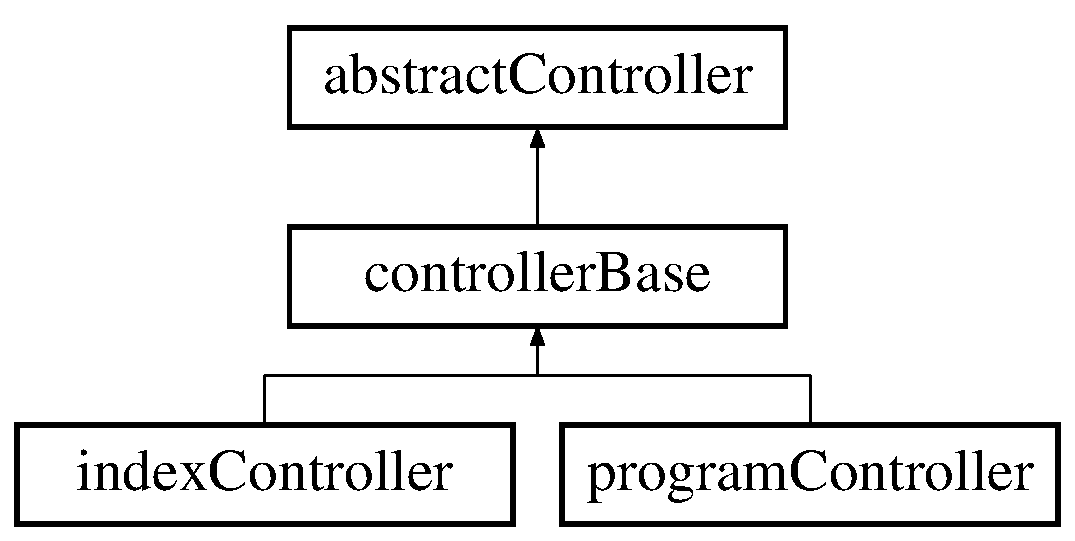
\includegraphics[height=3.000000cm]{classcontroller_base}
\end{center}
\end{figure}
\subsection*{Public Member Functions}
\begin{DoxyCompactItemize}
\item 
\hyperlink{classcontroller_base_a149eb92716c1084a935e04a8d95f7347}{index} ()
\item 
\hyperlink{classcontroller_base_a4be4055f3361d4800e16bc2e2e38cda6}{init} ()
\item 
\hyperlink{classcontroller_base_ac5e4cfad8999c9ab307b0eabded05722}{render\-View} (\$p\-\_\-s\-View= '\hyperlink{classcontroller_base_a149eb92716c1084a935e04a8d95f7347}{index}')
\end{DoxyCompactItemize}
\subsection*{Protected Member Functions}
\begin{DoxyCompactItemize}
\item 
\hyperlink{classcontroller_base_aa31bfdfbf8e089ed8054ff81aac51985}{set\-Db} (\hyperlink{classdb}{db} \$p\-\_\-o\-Db)
\item 
\hyperlink{classcontroller_base_aceb656ee5135578ab3a9947252caa772}{get\-Db} ()
\item 
\hyperlink{classcontroller_base_af1923f06f51143b20e3af00b02148c5d}{is\-Http\-Post} ()
\end{DoxyCompactItemize}
\subsection*{Additional Inherited Members}


\subsection{Member Function Documentation}
\hypertarget{classcontroller_base_aceb656ee5135578ab3a9947252caa772}{\index{controller\-Base@{controller\-Base}!get\-Db@{get\-Db}}
\index{get\-Db@{get\-Db}!controllerBase@{controller\-Base}}
\subsubsection[{get\-Db}]{\setlength{\rightskip}{0pt plus 5cm}get\-Db (
\begin{DoxyParamCaption}
{}
\end{DoxyParamCaption}
)\hspace{0.3cm}{\ttfamily [protected]}}}\label{classcontroller_base_aceb656ee5135578ab3a9947252caa772}
Getter for the database connection

\begin{DoxyReturn}{Returns}
db 
\end{DoxyReturn}
\hypertarget{classcontroller_base_a149eb92716c1084a935e04a8d95f7347}{\index{controller\-Base@{controller\-Base}!index@{index}}
\index{index@{index}!controllerBase@{controller\-Base}}
\subsubsection[{index}]{\setlength{\rightskip}{0pt plus 5cm}index (
\begin{DoxyParamCaption}
{}
\end{DoxyParamCaption}
)\hspace{0.3cm}{\ttfamily [abstract]}}}\label{classcontroller_base_a149eb92716c1084a935e04a8d95f7347}
all controllers must contain an index method \hypertarget{classcontroller_base_a4be4055f3361d4800e16bc2e2e38cda6}{\index{controller\-Base@{controller\-Base}!init@{init}}
\index{init@{init}!controllerBase@{controller\-Base}}
\subsubsection[{init}]{\setlength{\rightskip}{0pt plus 5cm}init (
\begin{DoxyParamCaption}
{}
\end{DoxyParamCaption}
)}}\label{classcontroller_base_a4be4055f3361d4800e16bc2e2e38cda6}
Initiates request handling and other basics common to all controllers and actions

\begin{DoxySeeAlso}{See Also}
\hyperlink{classabstract_controller}{abstract\-Controller} 
\end{DoxySeeAlso}
\hypertarget{classcontroller_base_af1923f06f51143b20e3af00b02148c5d}{\index{controller\-Base@{controller\-Base}!is\-Http\-Post@{is\-Http\-Post}}
\index{is\-Http\-Post@{is\-Http\-Post}!controllerBase@{controller\-Base}}
\subsubsection[{is\-Http\-Post}]{\setlength{\rightskip}{0pt plus 5cm}is\-Http\-Post (
\begin{DoxyParamCaption}
{}
\end{DoxyParamCaption}
)\hspace{0.3cm}{\ttfamily [protected]}}}\label{classcontroller_base_af1923f06f51143b20e3af00b02148c5d}
Determines whether the request method was H\-T\-T\-P-\/\-Post or not

\begin{DoxyReturn}{Returns}
bool True if H\-T\-T\-P-\/\-Post was used, false otherwise 
\end{DoxyReturn}
\hypertarget{classcontroller_base_ac5e4cfad8999c9ab307b0eabded05722}{\index{controller\-Base@{controller\-Base}!render\-View@{render\-View}}
\index{render\-View@{render\-View}!controllerBase@{controller\-Base}}
\subsubsection[{render\-View}]{\setlength{\rightskip}{0pt plus 5cm}render\-View (
\begin{DoxyParamCaption}
\item[{}]{\$p\-\_\-s\-View = {\ttfamily '{\bf index}'}}
\end{DoxyParamCaption}
)}}\label{classcontroller_base_ac5e4cfad8999c9ab307b0eabded05722}
Sends all content to the view to be rendered by the template


\begin{DoxyParams}[1]{Parameters}
string & {\em \$p\-\_\-s\-View} & The view to to call. Defaults to 'index' \\
\hline
\end{DoxyParams}
\begin{DoxyReturn}{Returns}
void 
\end{DoxyReturn}
\hypertarget{classcontroller_base_aa31bfdfbf8e089ed8054ff81aac51985}{\index{controller\-Base@{controller\-Base}!set\-Db@{set\-Db}}
\index{set\-Db@{set\-Db}!controllerBase@{controller\-Base}}
\subsubsection[{set\-Db}]{\setlength{\rightskip}{0pt plus 5cm}set\-Db (
\begin{DoxyParamCaption}
\item[{{\bf db}}]{\$p\-\_\-o\-Db}
\end{DoxyParamCaption}
)\hspace{0.3cm}{\ttfamily [protected]}}}\label{classcontroller_base_aa31bfdfbf8e089ed8054ff81aac51985}
Setter for the database connection


\begin{DoxyParams}[1]{Parameters}
db & {\em \$p\-\_\-o\-Db} & \\
\hline
\end{DoxyParams}


The documentation for this class was generated from the following file\-:\begin{DoxyCompactItemize}
\item 
/home/pa/web-\/projects/arbetsprov-\/project/arbetsprov.\-git/arbetsprov/application/controllers/controller\-Base.\-php\end{DoxyCompactItemize}

\hypertarget{classdb}{\section{db Class Reference}
\label{classdb}\index{db@{db}}
}
\subsection*{Public Member Functions}
\begin{DoxyCompactItemize}
\item 
\hyperlink{classdb_a095c5d389db211932136b53f25f39685}{\-\_\-\-\_\-construct} ()
\item 
\hyperlink{classdb_a1dfac6480d15a42a2c372ac0a4ea06ab}{set\-Attribute} (\$p\-\_\-s\-Attribute, \$p\-\_\-s\-Atribute\-Value)
\item 
\hyperlink{classdb_a5eba74d9e1df5186c10f0db10fb80e85}{prepare} (\$p\-\_\-s\-Sql)
\end{DoxyCompactItemize}
\subsection*{Data Fields}
\begin{DoxyCompactItemize}
\item 
\hypertarget{classdb_a85804db82403236e6751c7687139362e}{{\bfseries \$o\-Connection}}\label{classdb_a85804db82403236e6751c7687139362e}

\item 
\hypertarget{classdb_a143f69d339e788b0c2393f2134745e95}{{\bfseries \$o\-Stmt}}\label{classdb_a143f69d339e788b0c2393f2134745e95}

\end{DoxyCompactItemize}


\subsection{Constructor \& Destructor Documentation}
\hypertarget{classdb_a095c5d389db211932136b53f25f39685}{\index{db@{db}!\-\_\-\-\_\-construct@{\-\_\-\-\_\-construct}}
\index{\-\_\-\-\_\-construct@{\-\_\-\-\_\-construct}!db@{db}}
\subsubsection[{\-\_\-\-\_\-construct}]{\setlength{\rightskip}{0pt plus 5cm}\-\_\-\-\_\-construct (
\begin{DoxyParamCaption}
{}
\end{DoxyParamCaption}
)}}\label{classdb_a095c5d389db211932136b53f25f39685}
Connects to P\-D\-O -\/ Connection settings are located in config.\-ini

\begin{DoxyReturn}{Returns}
P\-D\-O 
\end{DoxyReturn}


\subsection{Member Function Documentation}
\hypertarget{classdb_a5eba74d9e1df5186c10f0db10fb80e85}{\index{db@{db}!prepare@{prepare}}
\index{prepare@{prepare}!db@{db}}
\subsubsection[{prepare}]{\setlength{\rightskip}{0pt plus 5cm}prepare (
\begin{DoxyParamCaption}
\item[{}]{\$p\-\_\-s\-Sql}
\end{DoxyParamCaption}
)}}\label{classdb_a5eba74d9e1df5186c10f0db10fb80e85}
Prepares a statement for execution and returns a statement object


\begin{DoxyParams}[1]{Parameters}
string & {\em \$p\-\_\-s\-Sql} & A valid S\-Q\-L-\/statement is expected \\
\hline
\end{DoxyParams}
\begin{DoxyReturn}{Returns}
P\-D\-O\-Statement 
\end{DoxyReturn}
\hypertarget{classdb_a1dfac6480d15a42a2c372ac0a4ea06ab}{\index{db@{db}!set\-Attribute@{set\-Attribute}}
\index{set\-Attribute@{set\-Attribute}!db@{db}}
\subsubsection[{set\-Attribute}]{\setlength{\rightskip}{0pt plus 5cm}set\-Attribute (
\begin{DoxyParamCaption}
\item[{}]{\$p\-\_\-s\-Attribute, }
\item[{}]{\$p\-\_\-s\-Atribute\-Value}
\end{DoxyParamCaption}
)}}\label{classdb_a1dfac6480d15a42a2c372ac0a4ea06ab}
Sets an attribute on the db handle


\begin{DoxyParams}[1]{Parameters}
string & {\em \$p\-\_\-s\-Attribute} & \\
\hline
string & {\em \$p\-\_\-s\-Atribute\-Value} & \\
\hline
\end{DoxyParams}
\begin{DoxyReturn}{Returns}
bool T\-R\-U\-E on success, F\-A\-L\-S\-E on failure 
\end{DoxyReturn}


The documentation for this class was generated from the following file\-:\begin{DoxyCompactItemize}
\item 
/home/pa/web-\/projects/arbetsprov-\/project/arbetsprov.\-git/arbetsprov/application/db.\-php\end{DoxyCompactItemize}

\hypertarget{classdebug}{\section{debug Class Reference}
\label{classdebug}\index{debug@{debug}}
}
\subsection*{Public Member Functions}
\begin{DoxyCompactItemize}
\item 
\hyperlink{classdebug_ae8684a77222708eb997247cd11b2a268}{\-\_\-\-\_\-construct} (\$p\-\_\-m\-To\-Inspect=false)
\end{DoxyCompactItemize}
\subsection*{Data Fields}
\begin{DoxyCompactItemize}
\item 
const \hyperlink{classdebug_a3948c042f5024ab0264a5413294eff6a}{N\-L} = \char`\"{}\textbackslash{}n\char`\"{}
\end{DoxyCompactItemize}


\subsection{Constructor \& Destructor Documentation}
\hypertarget{classdebug_ae8684a77222708eb997247cd11b2a268}{\index{debug@{debug}!\-\_\-\-\_\-construct@{\-\_\-\-\_\-construct}}
\index{\-\_\-\-\_\-construct@{\-\_\-\-\_\-construct}!debug@{debug}}
\subsubsection[{\-\_\-\-\_\-construct}]{\setlength{\rightskip}{0pt plus 5cm}\-\_\-\-\_\-construct (
\begin{DoxyParamCaption}
\item[{}]{\$p\-\_\-m\-To\-Inspect = {\ttfamily false}}
\end{DoxyParamCaption}
)}}\label{classdebug_ae8684a77222708eb997247cd11b2a268}
The constructor does the work of the class. Prints out the \$p\-\_\-m\-To\-Inspect using print\-\_\-r()


\begin{DoxyParams}[1]{Parameters}
mixed & {\em \$p\-\_\-m\-To\-Inspect} & Main data to display in the debug frame \\
\hline
\end{DoxyParams}


\subsection{Field Documentation}
\hypertarget{classdebug_a3948c042f5024ab0264a5413294eff6a}{\index{debug@{debug}!N\-L@{N\-L}}
\index{N\-L@{N\-L}!debug@{debug}}
\subsubsection[{N\-L}]{\setlength{\rightskip}{0pt plus 5cm}const N\-L = \char`\"{}\textbackslash{}n\char`\"{}}}\label{classdebug_a3948c042f5024ab0264a5413294eff6a}
new-\/line constant 

The documentation for this class was generated from the following file\-:\begin{DoxyCompactItemize}
\item 
/home/pa/web-\/projects/arbetsprov-\/project/arbetsprov.\-git/arbetsprov/application/lib/debug.\-php\end{DoxyCompactItemize}

\hypertarget{classindex_controller}{\section{index\-Controller Class Reference}
\label{classindex_controller}\index{index\-Controller@{index\-Controller}}
}
Inheritance diagram for index\-Controller\-:\begin{figure}[H]
\begin{center}
\leavevmode
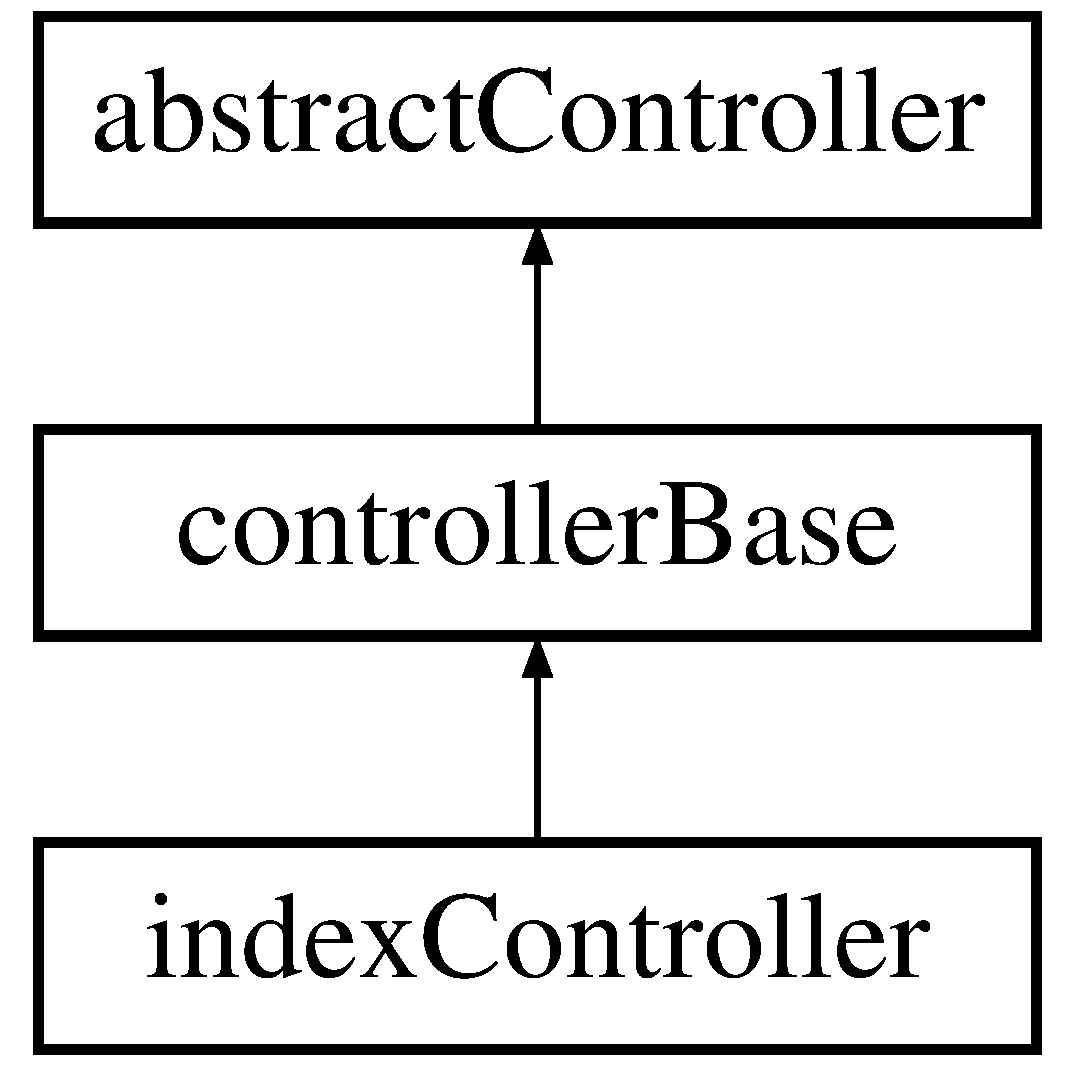
\includegraphics[height=3.000000cm]{classindex_controller}
\end{center}
\end{figure}
\subsection*{Public Member Functions}
\begin{DoxyCompactItemize}
\item 
\hyperlink{classindex_controller_a149eb92716c1084a935e04a8d95f7347}{index} ()
\end{DoxyCompactItemize}
\subsection*{Additional Inherited Members}


\subsection{Member Function Documentation}
\hypertarget{classindex_controller_a149eb92716c1084a935e04a8d95f7347}{\index{index\-Controller@{index\-Controller}!index@{index}}
\index{index@{index}!indexController@{index\-Controller}}
\subsubsection[{index}]{\setlength{\rightskip}{0pt plus 5cm}index (
\begin{DoxyParamCaption}
{}
\end{DoxyParamCaption}
)}}\label{classindex_controller_a149eb92716c1084a935e04a8d95f7347}
Main action delegation method of this class

\begin{DoxyReturn}{Returns}
void 
\end{DoxyReturn}


The documentation for this class was generated from the following file\-:\begin{DoxyCompactItemize}
\item 
/home/pa/web-\/projects/arbetsprov-\/project/arbetsprov.\-git/arbetsprov/application/controllers/index\-Controller.\-php\end{DoxyCompactItemize}

\hypertarget{class_page_fragment_base}{\section{Page\-Fragment\-Base Class Reference}
\label{class_page_fragment_base}\index{Page\-Fragment\-Base@{Page\-Fragment\-Base}}
}
Inheritance diagram for Page\-Fragment\-Base\-:\begin{figure}[H]
\begin{center}
\leavevmode
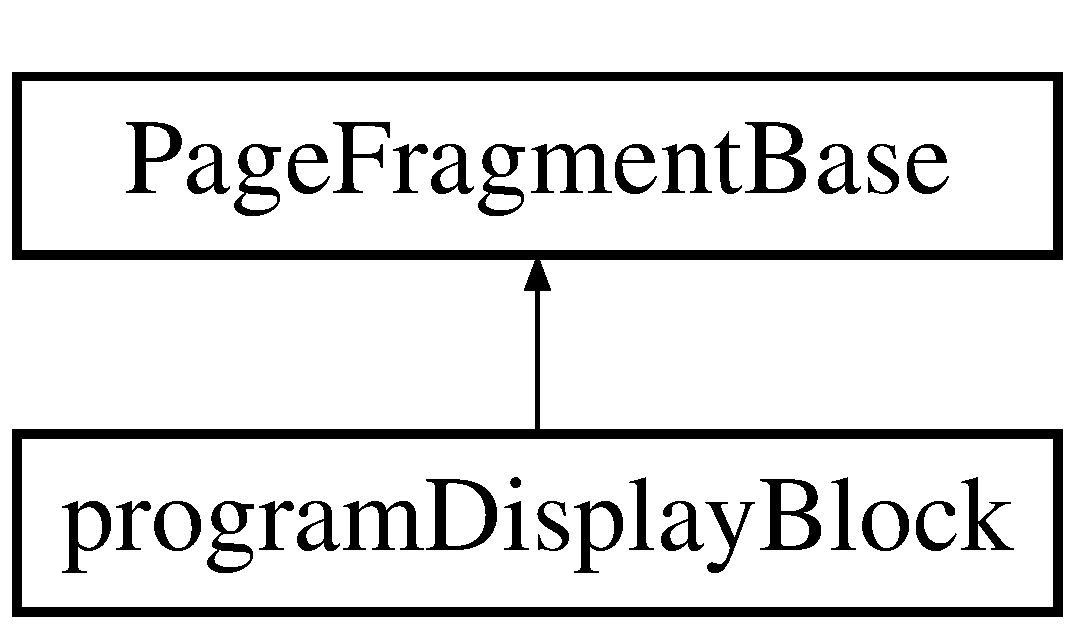
\includegraphics[height=2.000000cm]{class_page_fragment_base}
\end{center}
\end{figure}
\subsection*{Static Public Member Functions}
\begin{DoxyCompactItemize}
\item 
static \hyperlink{class_page_fragment_base_a0ebe09bd9f1f77ba934cb294606e010a}{append\-To\-Registry} (\$p\-\_\-s\-String\-To\-Add, \$p\-\_\-s\-Registry\-Key= 'main\-Content')
\item 
static \hyperlink{class_page_fragment_base_a86cc978fc5c3f2428380e6b9cad87b52}{get\-Registry} (\$p\-\_\-s\-Registry\-Key)
\item 
static \hyperlink{class_page_fragment_base_a5cb82f6d34119ef797d1820a5d3d585e}{set\-Registry} (\$p\-\_\-s\-Registry\-Key, \$p\-\_\-s\-Content)
\end{DoxyCompactItemize}
\subsection*{Data Fields}
\begin{DoxyCompactItemize}
\item 
const \hyperlink{class_page_fragment_base_a3948c042f5024ab0264a5413294eff6a}{N\-L} = \char`\"{}\textbackslash{}n\char`\"{}
\end{DoxyCompactItemize}


\subsection{Member Function Documentation}
\hypertarget{class_page_fragment_base_a0ebe09bd9f1f77ba934cb294606e010a}{\index{Page\-Fragment\-Base@{Page\-Fragment\-Base}!append\-To\-Registry@{append\-To\-Registry}}
\index{append\-To\-Registry@{append\-To\-Registry}!PageFragmentBase@{Page\-Fragment\-Base}}
\subsubsection[{append\-To\-Registry}]{\setlength{\rightskip}{0pt plus 5cm}static append\-To\-Registry (
\begin{DoxyParamCaption}
\item[{}]{\$p\-\_\-s\-String\-To\-Add, }
\item[{}]{\$p\-\_\-s\-Registry\-Key = {\ttfamily 'mainContent'}}
\end{DoxyParamCaption}
)\hspace{0.3cm}{\ttfamily [static]}}}\label{class_page_fragment_base_a0ebe09bd9f1f77ba934cb294606e010a}
Adds an extra string to the specified registry entry.

Intended to be called from methods needing to append strings to texts sent to the clients or for general display area build-\/up.


\begin{DoxyParams}[1]{Parameters}
string & {\em \$p\-\_\-s\-String\-To\-Add} & String to add to the registry \\
\hline
string & {\em \$p\-\_\-s\-Registry\-Key} & \hyperlink{class_registry}{Registry} key, may be defined in the calling methods, defaults to main\-Content \\
\hline
\end{DoxyParams}
\begin{DoxyReturn}{Returns}
bool Always true in lieu of void 
\end{DoxyReturn}
\hypertarget{class_page_fragment_base_a86cc978fc5c3f2428380e6b9cad87b52}{\index{Page\-Fragment\-Base@{Page\-Fragment\-Base}!get\-Registry@{get\-Registry}}
\index{get\-Registry@{get\-Registry}!PageFragmentBase@{Page\-Fragment\-Base}}
\subsubsection[{get\-Registry}]{\setlength{\rightskip}{0pt plus 5cm}static get\-Registry (
\begin{DoxyParamCaption}
\item[{}]{\$p\-\_\-s\-Registry\-Key}
\end{DoxyParamCaption}
)\hspace{0.3cm}{\ttfamily [static]}}}\label{class_page_fragment_base_a86cc978fc5c3f2428380e6b9cad87b52}
Fetches the content of a registry


\begin{DoxyParams}[1]{Parameters}
string & {\em \$p\-\_\-s\-Registry\-Key} & \\
\hline
\end{DoxyParams}
\begin{DoxyReturn}{Returns}
string \hyperlink{class_registry}{Registry} content, or empty string if not defined 
\end{DoxyReturn}
\hypertarget{class_page_fragment_base_a5cb82f6d34119ef797d1820a5d3d585e}{\index{Page\-Fragment\-Base@{Page\-Fragment\-Base}!set\-Registry@{set\-Registry}}
\index{set\-Registry@{set\-Registry}!PageFragmentBase@{Page\-Fragment\-Base}}
\subsubsection[{set\-Registry}]{\setlength{\rightskip}{0pt plus 5cm}static set\-Registry (
\begin{DoxyParamCaption}
\item[{}]{\$p\-\_\-s\-Registry\-Key, }
\item[{}]{\$p\-\_\-s\-Content}
\end{DoxyParamCaption}
)\hspace{0.3cm}{\ttfamily [static]}}}\label{class_page_fragment_base_a5cb82f6d34119ef797d1820a5d3d585e}
Sets (replaces) the content of a registry

The registry key is mandatory in order to minimize the risk of unintentionally replacing a registry


\begin{DoxyParams}[1]{Parameters}
string & {\em \$p\-\_\-s\-Registry\-Key} & \\
\hline
string & {\em \$p\-\_\-s\-Content} & \\
\hline
\end{DoxyParams}


\subsection{Field Documentation}
\hypertarget{class_page_fragment_base_a3948c042f5024ab0264a5413294eff6a}{\index{Page\-Fragment\-Base@{Page\-Fragment\-Base}!N\-L@{N\-L}}
\index{N\-L@{N\-L}!PageFragmentBase@{Page\-Fragment\-Base}}
\subsubsection[{N\-L}]{\setlength{\rightskip}{0pt plus 5cm}const N\-L = \char`\"{}\textbackslash{}n\char`\"{}}}\label{class_page_fragment_base_a3948c042f5024ab0264a5413294eff6a}
Constant for the newline character 

The documentation for this class was generated from the following file\-:\begin{DoxyCompactItemize}
\item 
/home/pa/web-\/projects/arbetsprov-\/project/arbetsprov.\-git/arbetsprov/application/page\-Fragments/page\-Fragment\-Base.\-php\end{DoxyCompactItemize}

\hypertarget{classprogram}{\section{program Class Reference}
\label{classprogram}\index{program@{program}}
}
\subsection*{Public Member Functions}
\begin{DoxyCompactItemize}
\item 
\hyperlink{classprogram_ac3f9d3c54d6fc31cf4ba8ee432250666}{get\-Pkey} ()
\item 
\hyperlink{classprogram_a2ac6ba685cbdbeaf1463acd2dda00723}{set\-Pkey} (\$p\-\_\-i\-Pkey)
\item 
\hyperlink{classprogram_a24d89b0ad05ea2e33626b1fc8ed59bc3}{get\-Date} ()
\item 
\hyperlink{classprogram_a975325739702b848dbe479b271eba40c}{set\-Date} (\$p\-\_\-s\-Date)
\item 
\hyperlink{classprogram_a568a7fafd601b520ff8c4bd91c962e29}{get\-Start\-Time} ()
\item 
\hyperlink{classprogram_a463e88d39545b8f5f3d191ee27bc95e7}{set\-Start\-Time} (\$p\-\_\-s\-Start\-Time)
\item 
\hyperlink{classprogram_a81ae59ce90d8e38356b0cad6851874e8}{get\-Lead\-Text} ()
\item 
\hyperlink{classprogram_a745b080e2d6c57a525c27e03ee61d184}{set\-Lead\-Text} (\$p\-\_\-s\-Lead\-Text)
\item 
\hyperlink{classprogram_a3d0963e68bb313b163a73f2803c64600}{get\-Name} ()
\item 
\hyperlink{classprogram_ab2d173090c606a8d0fff92a527707565}{set\-Name} (\$p\-\_\-s\-Name)
\item 
\hyperlink{classprogram_a770c51195d42a0a4933dc178bd6e2647}{get\-Bline} ()
\item 
\hyperlink{classprogram_a1bdde3b3633236fe5c3155cb9acaaf0d}{set\-Bline} (\$p\-\_\-s\-Byline)
\item 
\hyperlink{classprogram_a689e3214627e1e86671c39f506bb5ff5}{get\-Synopsis} ()
\item 
\hyperlink{classprogram_a9ff116e3d48acc95e9e53637dff65c21}{set\-Synopsis} (\$p\-\_\-s\-Synopsis)
\item 
\hyperlink{classprogram_accd14bda49a1044b4d8dd93f020f11ee}{get\-Url} ()
\item 
\hyperlink{classprogram_aa9f609d71b5936f6b51a5de0a86f4bec}{set\-Url} (\$p\-\_\-s\-Url)
\item 
\hyperlink{classprogram_a7c869f75ec8886cf1ece704ff07bdb6f}{\-\_\-\-\_\-construct} (\$p\-\_\-a\-Data=null)
\item 
\hyperlink{classprogram_a9c4738291eb554f8c6fbdaf85706bb47}{populate\-Data} (\$p\-\_\-a\-Data)
\end{DoxyCompactItemize}


\subsection{Constructor \& Destructor Documentation}
\hypertarget{classprogram_a7c869f75ec8886cf1ece704ff07bdb6f}{\index{program@{program}!\-\_\-\-\_\-construct@{\-\_\-\-\_\-construct}}
\index{\-\_\-\-\_\-construct@{\-\_\-\-\_\-construct}!program@{program}}
\subsubsection[{\-\_\-\-\_\-construct}]{\setlength{\rightskip}{0pt plus 5cm}\-\_\-\-\_\-construct (
\begin{DoxyParamCaption}
\item[{}]{\$p\-\_\-a\-Data = {\ttfamily null}}
\end{DoxyParamCaption}
)}}\label{classprogram_a7c869f75ec8886cf1ece704ff07bdb6f}
Constructor -\/ sets the member fields if relevant data is passed as parameter


\begin{DoxyParams}[1]{Parameters}
array & {\em \$p\-\_\-a\-Data} & Hash with data from some database \\
\hline
\end{DoxyParams}


\subsection{Member Function Documentation}
\hypertarget{classprogram_a770c51195d42a0a4933dc178bd6e2647}{\index{program@{program}!get\-Bline@{get\-Bline}}
\index{get\-Bline@{get\-Bline}!program@{program}}
\subsubsection[{get\-Bline}]{\setlength{\rightskip}{0pt plus 5cm}get\-Bline (
\begin{DoxyParamCaption}
{}
\end{DoxyParamCaption}
)}}\label{classprogram_a770c51195d42a0a4933dc178bd6e2647}
Getter for Bline

\begin{DoxyReturn}{Returns}
string \$s\-Bline 
\end{DoxyReturn}
\hypertarget{classprogram_a24d89b0ad05ea2e33626b1fc8ed59bc3}{\index{program@{program}!get\-Date@{get\-Date}}
\index{get\-Date@{get\-Date}!program@{program}}
\subsubsection[{get\-Date}]{\setlength{\rightskip}{0pt plus 5cm}get\-Date (
\begin{DoxyParamCaption}
{}
\end{DoxyParamCaption}
)}}\label{classprogram_a24d89b0ad05ea2e33626b1fc8ed59bc3}
Getter for date

\begin{DoxyReturn}{Returns}
string 
\end{DoxyReturn}
\hypertarget{classprogram_a81ae59ce90d8e38356b0cad6851874e8}{\index{program@{program}!get\-Lead\-Text@{get\-Lead\-Text}}
\index{get\-Lead\-Text@{get\-Lead\-Text}!program@{program}}
\subsubsection[{get\-Lead\-Text}]{\setlength{\rightskip}{0pt plus 5cm}get\-Lead\-Text (
\begin{DoxyParamCaption}
{}
\end{DoxyParamCaption}
)}}\label{classprogram_a81ae59ce90d8e38356b0cad6851874e8}
Getter for Leadtext

\begin{DoxyReturn}{Returns}
string \$s\-Lead\-Text 
\end{DoxyReturn}
\hypertarget{classprogram_a3d0963e68bb313b163a73f2803c64600}{\index{program@{program}!get\-Name@{get\-Name}}
\index{get\-Name@{get\-Name}!program@{program}}
\subsubsection[{get\-Name}]{\setlength{\rightskip}{0pt plus 5cm}get\-Name (
\begin{DoxyParamCaption}
{}
\end{DoxyParamCaption}
)}}\label{classprogram_a3d0963e68bb313b163a73f2803c64600}
Getter for Name

\begin{DoxyReturn}{Returns}
string \$s\-Name 
\end{DoxyReturn}
\hypertarget{classprogram_ac3f9d3c54d6fc31cf4ba8ee432250666}{\index{program@{program}!get\-Pkey@{get\-Pkey}}
\index{get\-Pkey@{get\-Pkey}!program@{program}}
\subsubsection[{get\-Pkey}]{\setlength{\rightskip}{0pt plus 5cm}get\-Pkey (
\begin{DoxyParamCaption}
{}
\end{DoxyParamCaption}
)}}\label{classprogram_ac3f9d3c54d6fc31cf4ba8ee432250666}
Getter for Pkey

\begin{DoxyReturn}{Returns}
int \$i\-Pkey 
\end{DoxyReturn}
\hypertarget{classprogram_a568a7fafd601b520ff8c4bd91c962e29}{\index{program@{program}!get\-Start\-Time@{get\-Start\-Time}}
\index{get\-Start\-Time@{get\-Start\-Time}!program@{program}}
\subsubsection[{get\-Start\-Time}]{\setlength{\rightskip}{0pt plus 5cm}get\-Start\-Time (
\begin{DoxyParamCaption}
{}
\end{DoxyParamCaption}
)}}\label{classprogram_a568a7fafd601b520ff8c4bd91c962e29}
Getter for Starttime

\begin{DoxyReturn}{Returns}
string \$s\-Start\-Time 
\end{DoxyReturn}
\hypertarget{classprogram_a689e3214627e1e86671c39f506bb5ff5}{\index{program@{program}!get\-Synopsis@{get\-Synopsis}}
\index{get\-Synopsis@{get\-Synopsis}!program@{program}}
\subsubsection[{get\-Synopsis}]{\setlength{\rightskip}{0pt plus 5cm}get\-Synopsis (
\begin{DoxyParamCaption}
{}
\end{DoxyParamCaption}
)}}\label{classprogram_a689e3214627e1e86671c39f506bb5ff5}
Getter for Synopsis

\begin{DoxyReturn}{Returns}
string \$s\-Synopsis 
\end{DoxyReturn}
\hypertarget{classprogram_accd14bda49a1044b4d8dd93f020f11ee}{\index{program@{program}!get\-Url@{get\-Url}}
\index{get\-Url@{get\-Url}!program@{program}}
\subsubsection[{get\-Url}]{\setlength{\rightskip}{0pt plus 5cm}get\-Url (
\begin{DoxyParamCaption}
{}
\end{DoxyParamCaption}
)}}\label{classprogram_accd14bda49a1044b4d8dd93f020f11ee}
Getter for Url

\begin{DoxyReturn}{Returns}
string \$s\-Url 
\end{DoxyReturn}
\hypertarget{classprogram_a9c4738291eb554f8c6fbdaf85706bb47}{\index{program@{program}!populate\-Data@{populate\-Data}}
\index{populate\-Data@{populate\-Data}!program@{program}}
\subsubsection[{populate\-Data}]{\setlength{\rightskip}{0pt plus 5cm}populate\-Data (
\begin{DoxyParamCaption}
\item[{}]{\$p\-\_\-a\-Data}
\end{DoxyParamCaption}
)}}\label{classprogram_a9c4738291eb554f8c6fbdaf85706bb47}
Populates the list data fields


\begin{DoxyParams}[1]{Parameters}
array & {\em \$p\-\_\-a\-Data} & Hash with key =$>$ value pairs \\
\hline
\end{DoxyParams}
\begin{DoxyReturn}{Returns}
int Number of populated member fields 
\end{DoxyReturn}
\hypertarget{classprogram_a1bdde3b3633236fe5c3155cb9acaaf0d}{\index{program@{program}!set\-Bline@{set\-Bline}}
\index{set\-Bline@{set\-Bline}!program@{program}}
\subsubsection[{set\-Bline}]{\setlength{\rightskip}{0pt plus 5cm}set\-Bline (
\begin{DoxyParamCaption}
\item[{}]{\$p\-\_\-s\-Byline}
\end{DoxyParamCaption}
)}}\label{classprogram_a1bdde3b3633236fe5c3155cb9acaaf0d}
Setter for Bline


\begin{DoxyParams}[1]{Parameters}
string & {\em \$p\-\_\-s\-Bline} & \\
\hline
\end{DoxyParams}
\hypertarget{classprogram_a975325739702b848dbe479b271eba40c}{\index{program@{program}!set\-Date@{set\-Date}}
\index{set\-Date@{set\-Date}!program@{program}}
\subsubsection[{set\-Date}]{\setlength{\rightskip}{0pt plus 5cm}set\-Date (
\begin{DoxyParamCaption}
\item[{}]{\$p\-\_\-s\-Date}
\end{DoxyParamCaption}
)}}\label{classprogram_a975325739702b848dbe479b271eba40c}
Setter for date


\begin{DoxyParams}[1]{Parameters}
string & {\em \$p\-\_\-s\-Date} & \\
\hline
\end{DoxyParams}
\hypertarget{classprogram_a745b080e2d6c57a525c27e03ee61d184}{\index{program@{program}!set\-Lead\-Text@{set\-Lead\-Text}}
\index{set\-Lead\-Text@{set\-Lead\-Text}!program@{program}}
\subsubsection[{set\-Lead\-Text}]{\setlength{\rightskip}{0pt plus 5cm}set\-Lead\-Text (
\begin{DoxyParamCaption}
\item[{}]{\$p\-\_\-s\-Lead\-Text}
\end{DoxyParamCaption}
)}}\label{classprogram_a745b080e2d6c57a525c27e03ee61d184}
Setter for Lead\-Text


\begin{DoxyParams}[1]{Parameters}
string & {\em \$s\-Lead\-Text} & \\
\hline
\end{DoxyParams}
\hypertarget{classprogram_ab2d173090c606a8d0fff92a527707565}{\index{program@{program}!set\-Name@{set\-Name}}
\index{set\-Name@{set\-Name}!program@{program}}
\subsubsection[{set\-Name}]{\setlength{\rightskip}{0pt plus 5cm}set\-Name (
\begin{DoxyParamCaption}
\item[{}]{\$p\-\_\-s\-Name}
\end{DoxyParamCaption}
)}}\label{classprogram_ab2d173090c606a8d0fff92a527707565}
Setter for Name


\begin{DoxyParams}[1]{Parameters}
string & {\em \$s\-Name} & \\
\hline
\end{DoxyParams}
\hypertarget{classprogram_a2ac6ba685cbdbeaf1463acd2dda00723}{\index{program@{program}!set\-Pkey@{set\-Pkey}}
\index{set\-Pkey@{set\-Pkey}!program@{program}}
\subsubsection[{set\-Pkey}]{\setlength{\rightskip}{0pt plus 5cm}set\-Pkey (
\begin{DoxyParamCaption}
\item[{}]{\$p\-\_\-i\-Pkey}
\end{DoxyParamCaption}
)}}\label{classprogram_a2ac6ba685cbdbeaf1463acd2dda00723}
Setter for Pkey


\begin{DoxyParams}[1]{Parameters}
int & {\em \$p\-\_\-i\-Pkey} & \\
\hline
\end{DoxyParams}
\hypertarget{classprogram_a463e88d39545b8f5f3d191ee27bc95e7}{\index{program@{program}!set\-Start\-Time@{set\-Start\-Time}}
\index{set\-Start\-Time@{set\-Start\-Time}!program@{program}}
\subsubsection[{set\-Start\-Time}]{\setlength{\rightskip}{0pt plus 5cm}set\-Start\-Time (
\begin{DoxyParamCaption}
\item[{}]{\$p\-\_\-s\-Start\-Time}
\end{DoxyParamCaption}
)}}\label{classprogram_a463e88d39545b8f5f3d191ee27bc95e7}
Setter for Start\-Time


\begin{DoxyParams}[1]{Parameters}
time & {\em \$p\-\_\-s\-Start\-Time} & \\
\hline
\end{DoxyParams}
\hypertarget{classprogram_a9ff116e3d48acc95e9e53637dff65c21}{\index{program@{program}!set\-Synopsis@{set\-Synopsis}}
\index{set\-Synopsis@{set\-Synopsis}!program@{program}}
\subsubsection[{set\-Synopsis}]{\setlength{\rightskip}{0pt plus 5cm}set\-Synopsis (
\begin{DoxyParamCaption}
\item[{}]{\$p\-\_\-s\-Synopsis}
\end{DoxyParamCaption}
)}}\label{classprogram_a9ff116e3d48acc95e9e53637dff65c21}
Setter for Synopsis


\begin{DoxyParams}[1]{Parameters}
string & {\em \$s\-Synopsis} & \\
\hline
\end{DoxyParams}
\hypertarget{classprogram_aa9f609d71b5936f6b51a5de0a86f4bec}{\index{program@{program}!set\-Url@{set\-Url}}
\index{set\-Url@{set\-Url}!program@{program}}
\subsubsection[{set\-Url}]{\setlength{\rightskip}{0pt plus 5cm}set\-Url (
\begin{DoxyParamCaption}
\item[{}]{\$p\-\_\-s\-Url}
\end{DoxyParamCaption}
)}}\label{classprogram_aa9f609d71b5936f6b51a5de0a86f4bec}
Setter for Url


\begin{DoxyParams}[1]{Parameters}
string & {\em \$s\-Url} & \\
\hline
\end{DoxyParams}


The documentation for this class was generated from the following file\-:\begin{DoxyCompactItemize}
\item 
/home/pa/web-\/projects/arbetsprov-\/project/arbetsprov.\-git/arbetsprov/application/models/program.\-php\end{DoxyCompactItemize}

\hypertarget{classprogram_controller}{\section{program\-Controller Class Reference}
\label{classprogram_controller}\index{program\-Controller@{program\-Controller}}
}
Inheritance diagram for program\-Controller\-:\begin{figure}[H]
\begin{center}
\leavevmode
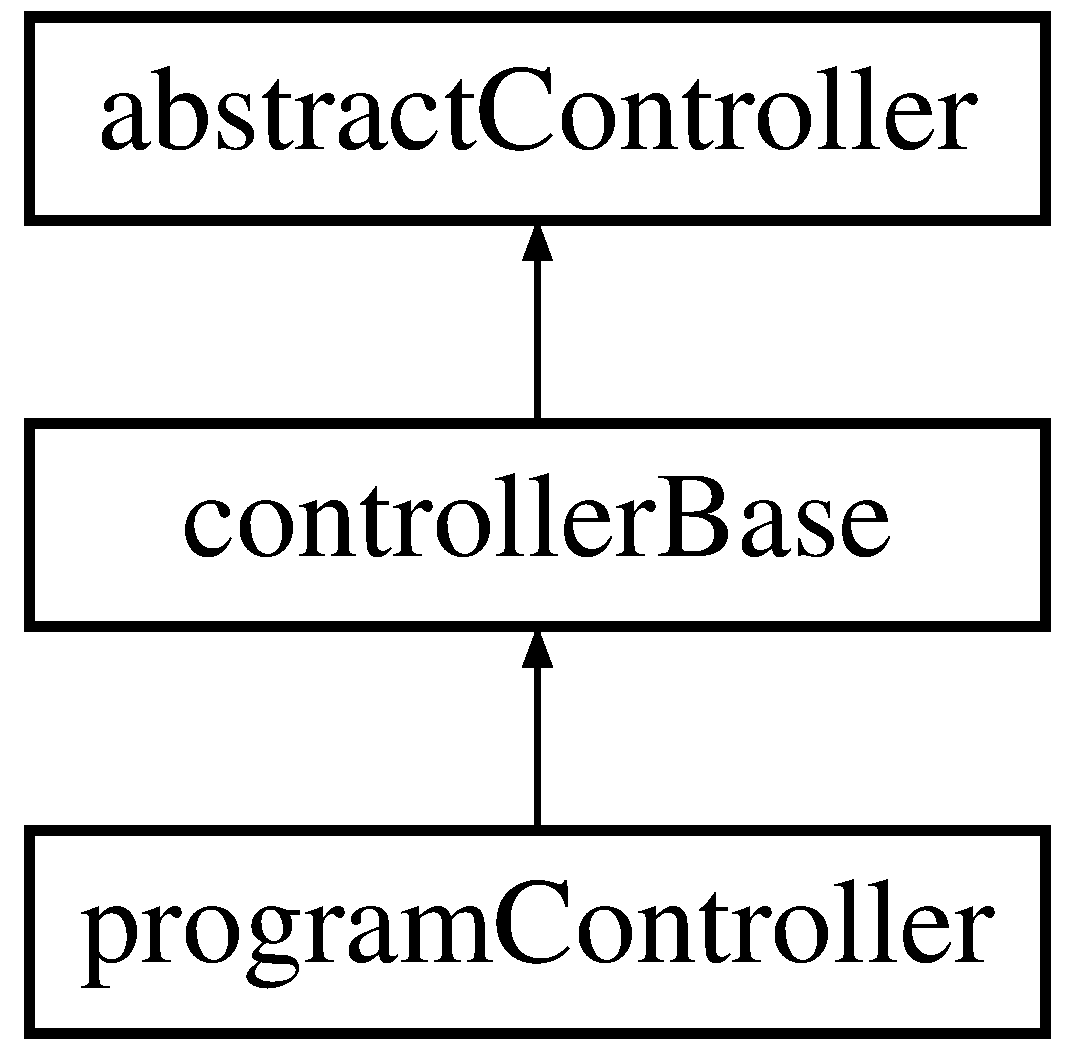
\includegraphics[height=3.000000cm]{classprogram_controller}
\end{center}
\end{figure}
\subsection*{Public Member Functions}
\begin{DoxyCompactItemize}
\item 
\hyperlink{classprogram_controller_a149eb92716c1084a935e04a8d95f7347}{index} ()
\item 
\hyperlink{classprogram_controller_a92fb4a09ef2b90bb7989581130af0570}{program\-List} (\$p\-\_\-a\-Req\-Params)
\item 
\hyperlink{classprogram_controller_ab1b9db62e2662a2ad874b1817123659a}{program\-Add} ()
\item 
\hyperlink{classprogram_controller_a97a2d8b5d4a9f4bb31583bc8cd583bf1}{program\-Update} (\$p\-\_\-a\-Req\-Params)
\item 
\hyperlink{classprogram_controller_af04444cdcd982905cc5cfd23d5845d5c}{program\-Delete} ()
\item 
\hyperlink{classprogram_controller_a81ac253885e630f788e56b308cc5769e}{program\-Xml} ()
\item 
\hyperlink{classprogram_controller_a43993da6cb1ef597d6fbacc778133112}{validate\-Post\-Data} (\$p\-\_\-a\-Data)
\end{DoxyCompactItemize}
\subsection*{Additional Inherited Members}


\subsection{Member Function Documentation}
\hypertarget{classprogram_controller_a149eb92716c1084a935e04a8d95f7347}{\index{program\-Controller@{program\-Controller}!index@{index}}
\index{index@{index}!programController@{program\-Controller}}
\subsubsection[{index}]{\setlength{\rightskip}{0pt plus 5cm}index (
\begin{DoxyParamCaption}
{}
\end{DoxyParamCaption}
)}}\label{classprogram_controller_a149eb92716c1084a935e04a8d95f7347}
Main action delegation method of this class

\begin{DoxyReturn}{Returns}
void 
\end{DoxyReturn}
\hypertarget{classprogram_controller_ab1b9db62e2662a2ad874b1817123659a}{\index{program\-Controller@{program\-Controller}!program\-Add@{program\-Add}}
\index{program\-Add@{program\-Add}!programController@{program\-Controller}}
\subsubsection[{program\-Add}]{\setlength{\rightskip}{0pt plus 5cm}program\-Add (
\begin{DoxyParamCaption}
{}
\end{DoxyParamCaption}
)}}\label{classprogram_controller_ab1b9db62e2662a2ad874b1817123659a}
Handles the adding of new programs Corresponds to the url -\/ /program/add/

return void \hypertarget{classprogram_controller_af04444cdcd982905cc5cfd23d5845d5c}{\index{program\-Controller@{program\-Controller}!program\-Delete@{program\-Delete}}
\index{program\-Delete@{program\-Delete}!programController@{program\-Controller}}
\subsubsection[{program\-Delete}]{\setlength{\rightskip}{0pt plus 5cm}program\-Delete (
\begin{DoxyParamCaption}
{}
\end{DoxyParamCaption}
)}}\label{classprogram_controller_af04444cdcd982905cc5cfd23d5845d5c}
Hamdles the delete action

return void \hypertarget{classprogram_controller_a92fb4a09ef2b90bb7989581130af0570}{\index{program\-Controller@{program\-Controller}!program\-List@{program\-List}}
\index{program\-List@{program\-List}!programController@{program\-Controller}}
\subsubsection[{program\-List}]{\setlength{\rightskip}{0pt plus 5cm}program\-List (
\begin{DoxyParamCaption}
\item[{}]{\$p\-\_\-a\-Req\-Params}
\end{DoxyParamCaption}
)}}\label{classprogram_controller_a92fb4a09ef2b90bb7989581130af0570}
Handles the listing of programdata Corresponds to the url /program/list/


\begin{DoxyParams}[1]{Parameters}
array & {\em \$p\-\_\-a\-Req\-Params} & Request parameters as exploded on / by the action delegation method \\
\hline
\end{DoxyParams}
\hypertarget{classprogram_controller_a97a2d8b5d4a9f4bb31583bc8cd583bf1}{\index{program\-Controller@{program\-Controller}!program\-Update@{program\-Update}}
\index{program\-Update@{program\-Update}!programController@{program\-Controller}}
\subsubsection[{program\-Update}]{\setlength{\rightskip}{0pt plus 5cm}program\-Update (
\begin{DoxyParamCaption}
\item[{}]{\$p\-\_\-a\-Req\-Params}
\end{DoxyParamCaption}
)}}\label{classprogram_controller_a97a2d8b5d4a9f4bb31583bc8cd583bf1}
Handles the updating of programdata Corresponds to the url /program/update/nn


\begin{DoxyParams}[1]{Parameters}
array & {\em \$p\-\_\-a\-Req\-Params} & Request parameters as exploded on / by the action delegation method \\
\hline
\end{DoxyParams}
\begin{DoxyReturn}{Returns}
void 
\end{DoxyReturn}
\hypertarget{classprogram_controller_a81ac253885e630f788e56b308cc5769e}{\index{program\-Controller@{program\-Controller}!program\-Xml@{program\-Xml}}
\index{program\-Xml@{program\-Xml}!programController@{program\-Controller}}
\subsubsection[{program\-Xml}]{\setlength{\rightskip}{0pt plus 5cm}program\-Xml (
\begin{DoxyParamCaption}
{}
\end{DoxyParamCaption}
)}}\label{classprogram_controller_a81ac253885e630f788e56b308cc5769e}
Handles the request to view programdata as X\-M\-L Corresponds to the url /program/xml/

return void \hypertarget{classprogram_controller_a43993da6cb1ef597d6fbacc778133112}{\index{program\-Controller@{program\-Controller}!validate\-Post\-Data@{validate\-Post\-Data}}
\index{validate\-Post\-Data@{validate\-Post\-Data}!programController@{program\-Controller}}
\subsubsection[{validate\-Post\-Data}]{\setlength{\rightskip}{0pt plus 5cm}validate\-Post\-Data (
\begin{DoxyParamCaption}
\item[{}]{\$p\-\_\-a\-Data}
\end{DoxyParamCaption}
)}}\label{classprogram_controller_a43993da6cb1ef597d6fbacc778133112}
Checks for missing fields when adding/updating


\begin{DoxyParams}[1]{Parameters}
array & {\em \$p\-\_\-a\-Data} & \\
\hline
\end{DoxyParams}
\begin{DoxyReturn}{Returns}
bool True if no fields are empty, false otherwise 
\end{DoxyReturn}


The documentation for this class was generated from the following file\-:\begin{DoxyCompactItemize}
\item 
/home/pa/web-\/projects/arbetsprov-\/project/arbetsprov.\-git/arbetsprov/application/controllers/program\-Controller.\-php\end{DoxyCompactItemize}

\hypertarget{classprogram_display_block}{\section{program\-Display\-Block Class Reference}
\label{classprogram_display_block}\index{program\-Display\-Block@{program\-Display\-Block}}
}
Inheritance diagram for program\-Display\-Block\-:\begin{figure}[H]
\begin{center}
\leavevmode
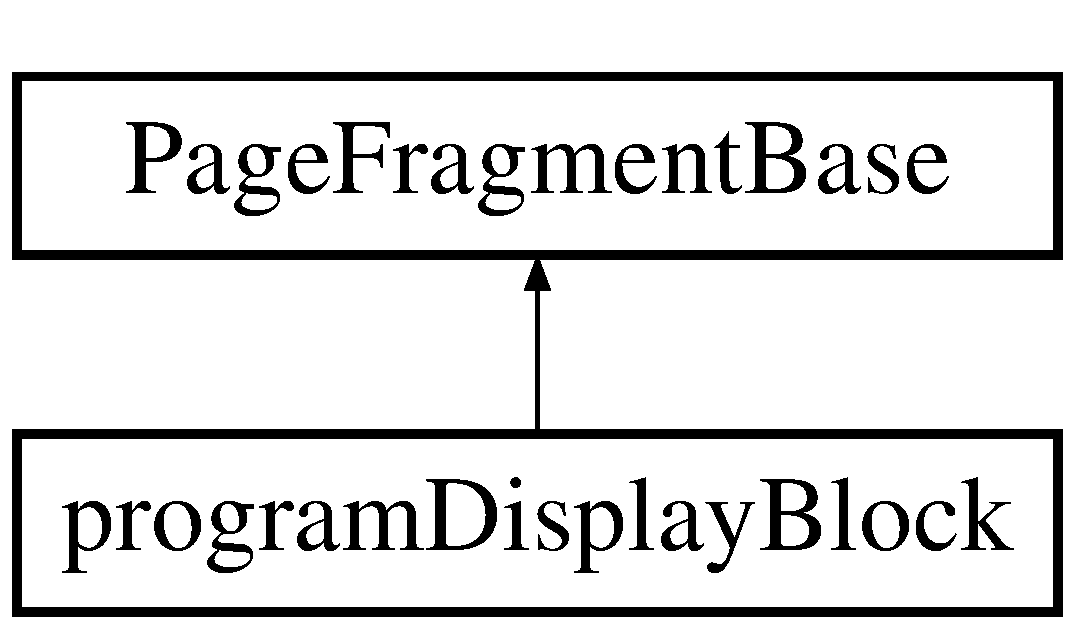
\includegraphics[height=2.000000cm]{classprogram_display_block}
\end{center}
\end{figure}
\subsection*{Public Member Functions}
\begin{DoxyCompactItemize}
\item 
\hyperlink{classprogram_display_block_acf91adc69deb5749f1747360574888d6}{render\-Table} (Array\-Object \$p\-\_\-o\-List\-Data)
\item 
\hyperlink{classprogram_display_block_ac97675c9ddbae0b41ae67ebce4735723}{render\-Editform} (\hyperlink{classprogram}{program} \$p\-\_\-o\-Program)
\item 
\hyperlink{classprogram_display_block_a60673ef5b741a95c4d513088f97d9cbc}{render\-Addform} ()
\item 
\hyperlink{classprogram_display_block_a7dcb164b59f7680e7e350340337cb168}{render\-Delete\-Form} (\$p\-\_\-i\-Key)
\end{DoxyCompactItemize}
\subsection*{Additional Inherited Members}


\subsection{Member Function Documentation}
\hypertarget{classprogram_display_block_a60673ef5b741a95c4d513088f97d9cbc}{\index{program\-Display\-Block@{program\-Display\-Block}!render\-Addform@{render\-Addform}}
\index{render\-Addform@{render\-Addform}!programDisplayBlock@{program\-Display\-Block}}
\subsubsection[{render\-Addform}]{\setlength{\rightskip}{0pt plus 5cm}render\-Addform (
\begin{DoxyParamCaption}
{}
\end{DoxyParamCaption}
)}}\label{classprogram_display_block_a60673ef5b741a95c4d513088f97d9cbc}
Renders the add form

\begin{DoxyReturn}{Returns}
string html code 
\end{DoxyReturn}
\hypertarget{classprogram_display_block_a7dcb164b59f7680e7e350340337cb168}{\index{program\-Display\-Block@{program\-Display\-Block}!render\-Delete\-Form@{render\-Delete\-Form}}
\index{render\-Delete\-Form@{render\-Delete\-Form}!programDisplayBlock@{program\-Display\-Block}}
\subsubsection[{render\-Delete\-Form}]{\setlength{\rightskip}{0pt plus 5cm}render\-Delete\-Form (
\begin{DoxyParamCaption}
\item[{}]{\$p\-\_\-i\-Key}
\end{DoxyParamCaption}
)}}\label{classprogram_display_block_a7dcb164b59f7680e7e350340337cb168}
Renders the delete form


\begin{DoxyParams}[1]{Parameters}
int & {\em \$p\-\_\-i\-Key} & Id key for the row to delete \\
\hline
\end{DoxyParams}
\begin{DoxyReturn}{Returns}
string html code 
\end{DoxyReturn}
\hypertarget{classprogram_display_block_ac97675c9ddbae0b41ae67ebce4735723}{\index{program\-Display\-Block@{program\-Display\-Block}!render\-Editform@{render\-Editform}}
\index{render\-Editform@{render\-Editform}!programDisplayBlock@{program\-Display\-Block}}
\subsubsection[{render\-Editform}]{\setlength{\rightskip}{0pt plus 5cm}render\-Editform (
\begin{DoxyParamCaption}
\item[{{\bf program}}]{\$p\-\_\-o\-Program}
\end{DoxyParamCaption}
)}}\label{classprogram_display_block_ac97675c9ddbae0b41ae67ebce4735723}
Renders the edit form


\begin{DoxyParams}[1]{Parameters}
program & {\em \$p\-\_\-o\-Program} & \\
\hline
\end{DoxyParams}
\begin{DoxyReturn}{Returns}
string html code 
\end{DoxyReturn}
\hypertarget{classprogram_display_block_acf91adc69deb5749f1747360574888d6}{\index{program\-Display\-Block@{program\-Display\-Block}!render\-Table@{render\-Table}}
\index{render\-Table@{render\-Table}!programDisplayBlock@{program\-Display\-Block}}
\subsubsection[{render\-Table}]{\setlength{\rightskip}{0pt plus 5cm}render\-Table (
\begin{DoxyParamCaption}
\item[{Array\-Object}]{\$p\-\_\-o\-List\-Data}
\end{DoxyParamCaption}
)}}\label{classprogram_display_block_acf91adc69deb5749f1747360574888d6}
Renders the data list table


\begin{DoxyParams}[1]{Parameters}
Array\-Object & {\em \$p\-\_\-o\-List\-Data} & \\
\hline
\end{DoxyParams}
\begin{DoxyReturn}{Returns}
string Html code 
\end{DoxyReturn}


The documentation for this class was generated from the following file\-:\begin{DoxyCompactItemize}
\item 
/home/pa/web-\/projects/arbetsprov-\/project/arbetsprov.\-git/arbetsprov/application/page\-Fragments/display\-Blocks/program\-Display\-Block.\-php\end{DoxyCompactItemize}

\hypertarget{class_registry}{\section{Registry Class Reference}
\label{class_registry}\index{Registry@{Registry}}
}
Inheritance diagram for Registry\-:\begin{figure}[H]
\begin{center}
\leavevmode
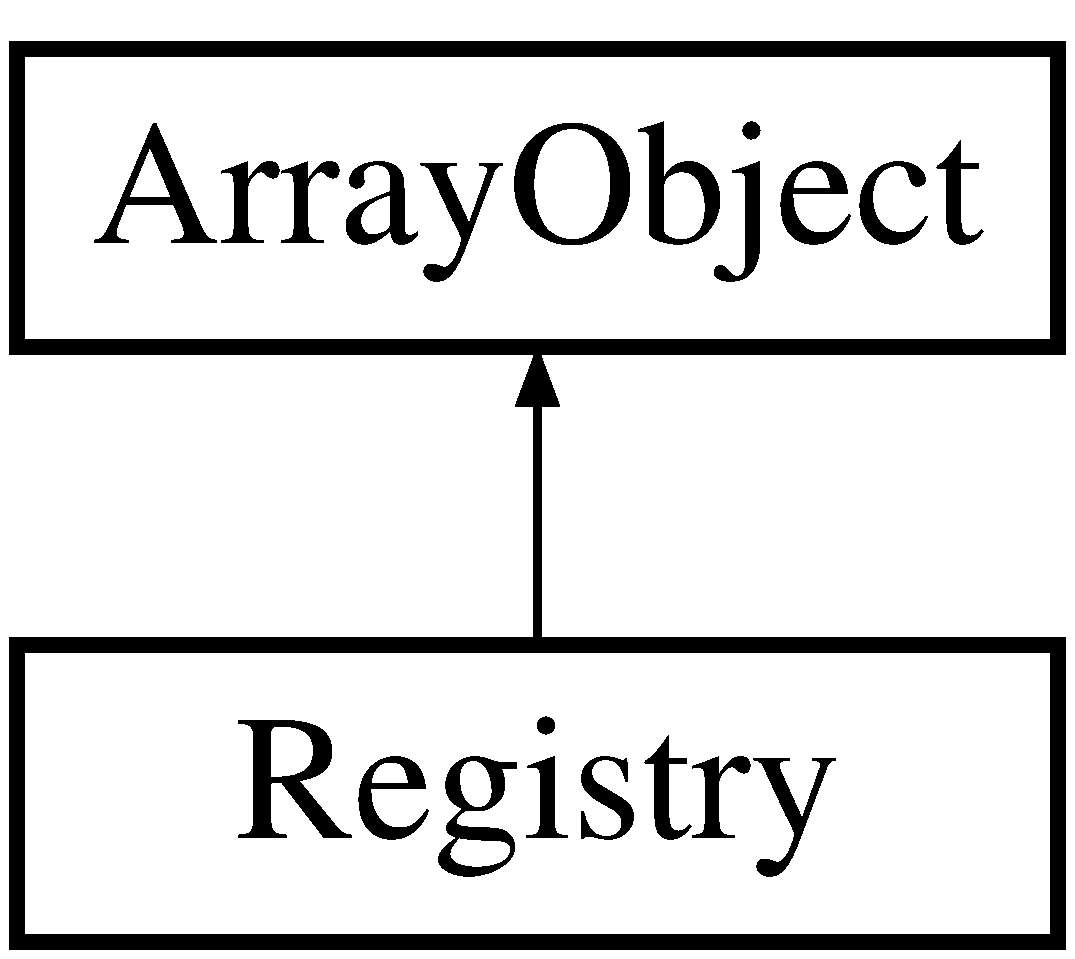
\includegraphics[height=2.000000cm]{class_registry}
\end{center}
\end{figure}
\subsection*{Public Member Functions}
\begin{DoxyCompactItemize}
\item 
\hyperlink{class_registry_a72d07723c008ae1b9e7e3ff006dc40aa}{offset\-Exists} (\$p\-\_\-s\-Index)
\end{DoxyCompactItemize}
\subsection*{Static Public Member Functions}
\begin{DoxyCompactItemize}
\item 
static \hyperlink{class_registry_ac93fbec81f07e5d15f80db907e63dc10}{get\-Instance} ()
\item 
static \hyperlink{class_registry_ae3e77c45ddd8ee222fa2020c25224e28}{set\-Instance} (\$p\-\_\-o\-Registry)
\item 
static \hyperlink{class_registry_a2fa3f8432843f2d4a983039da16d56b2}{set\-Class\-Name} (\$p\-\_\-s\-Class\-Name= '\hyperlink{class_registry}{Registry}')
\item 
static \hyperlink{class_registry_afd3d1c0ff850d37f8fe451be604735f3}{unset\-Instance} ()
\item 
static \hyperlink{class_registry_a624be586dc28014cd2c189beb7060bba}{get} (\$p\-\_\-s\-Index)
\item 
static \hyperlink{class_registry_adfd9ba1232394d791088a0310cd394f6}{set} (\$p\-\_\-s\-Index, \$p\-\_\-m\-Value)
\item 
static \hyperlink{class_registry_a2e51a1575dbd47b8e76da8cb7df36d3d}{is\-Registered} (\$p\-\_\-s\-Index)
\end{DoxyCompactItemize}
\subsection*{Static Protected Member Functions}
\begin{DoxyCompactItemize}
\item 
static \hyperlink{class_registry_a9f0be6ae273d3669e11c29910a0be338}{init} ()
\end{DoxyCompactItemize}


\subsection{Member Function Documentation}
\hypertarget{class_registry_a624be586dc28014cd2c189beb7060bba}{\index{Registry@{Registry}!get@{get}}
\index{get@{get}!Registry@{Registry}}
\subsubsection[{get}]{\setlength{\rightskip}{0pt plus 5cm}static get (
\begin{DoxyParamCaption}
\item[{}]{\$p\-\_\-s\-Index}
\end{DoxyParamCaption}
)\hspace{0.3cm}{\ttfamily [static]}}}\label{class_registry_a624be586dc28014cd2c189beb7060bba}
Getter method, synonymous to offset\-Get()


\begin{DoxyParams}[1]{Parameters}
string & {\em \$p\-\_\-s\-Index} & -\/ get the value associated with \$index \\
\hline
\end{DoxyParams}
\begin{DoxyReturn}{Returns}
mixed 
\end{DoxyReturn}

\begin{DoxyExceptions}{Exceptions}
{\em Exception} & if no entry is registerd for \$index. \\
\hline
\end{DoxyExceptions}
\hypertarget{class_registry_ac93fbec81f07e5d15f80db907e63dc10}{\index{Registry@{Registry}!get\-Instance@{get\-Instance}}
\index{get\-Instance@{get\-Instance}!Registry@{Registry}}
\subsubsection[{get\-Instance}]{\setlength{\rightskip}{0pt plus 5cm}static get\-Instance (
\begin{DoxyParamCaption}
{}
\end{DoxyParamCaption}
)\hspace{0.3cm}{\ttfamily [static]}}}\label{class_registry_ac93fbec81f07e5d15f80db907e63dc10}
Getter for \hyperlink{class_registry}{Registry}

\begin{DoxyReturn}{Returns}
\hyperlink{class_registry}{Registry} 
\end{DoxyReturn}
\hypertarget{class_registry_a9f0be6ae273d3669e11c29910a0be338}{\index{Registry@{Registry}!init@{init}}
\index{init@{init}!Registry@{Registry}}
\subsubsection[{init}]{\setlength{\rightskip}{0pt plus 5cm}static init (
\begin{DoxyParamCaption}
{}
\end{DoxyParamCaption}
)\hspace{0.3cm}{\ttfamily [static]}, {\ttfamily [protected]}}}\label{class_registry_a9f0be6ae273d3669e11c29910a0be338}
Initialize this instance

\begin{DoxyReturn}{Returns}
void 
\end{DoxyReturn}
\hypertarget{class_registry_a2e51a1575dbd47b8e76da8cb7df36d3d}{\index{Registry@{Registry}!is\-Registered@{is\-Registered}}
\index{is\-Registered@{is\-Registered}!Registry@{Registry}}
\subsubsection[{is\-Registered}]{\setlength{\rightskip}{0pt plus 5cm}static is\-Registered (
\begin{DoxyParamCaption}
\item[{}]{\$p\-\_\-s\-Index}
\end{DoxyParamCaption}
)\hspace{0.3cm}{\ttfamily [static]}}}\label{class_registry_a2e51a1575dbd47b8e76da8cb7df36d3d}
Checks if a value is registered, synonymous to \hyperlink{class_registry_a72d07723c008ae1b9e7e3ff006dc40aa}{offset\-Exists()}


\begin{DoxyParams}[1]{Parameters}
string & {\em \$p\-\_\-s\-Index} & \\
\hline
\end{DoxyParams}
\begin{DoxyReturn}{Returns}
bool True if \$p\-\_\-s\-Index is a named value in the registry, false otherwise 
\end{DoxyReturn}
\hypertarget{class_registry_a72d07723c008ae1b9e7e3ff006dc40aa}{\index{Registry@{Registry}!offset\-Exists@{offset\-Exists}}
\index{offset\-Exists@{offset\-Exists}!Registry@{Registry}}
\subsubsection[{offset\-Exists}]{\setlength{\rightskip}{0pt plus 5cm}offset\-Exists (
\begin{DoxyParamCaption}
\item[{}]{\$p\-\_\-s\-Index}
\end{DoxyParamCaption}
)}}\label{class_registry_a72d07723c008ae1b9e7e3ff006dc40aa}
Wrapper method for offset\-Exists


\begin{DoxyParams}[1]{Parameters}
string & {\em \$index} & \\
\hline
\end{DoxyParams}
\begin{DoxyReturn}{Returns}
mixed 
\end{DoxyReturn}
\hypertarget{class_registry_adfd9ba1232394d791088a0310cd394f6}{\index{Registry@{Registry}!set@{set}}
\index{set@{set}!Registry@{Registry}}
\subsubsection[{set}]{\setlength{\rightskip}{0pt plus 5cm}static set (
\begin{DoxyParamCaption}
\item[{}]{\$p\-\_\-s\-Index, }
\item[{}]{\$p\-\_\-m\-Value}
\end{DoxyParamCaption}
)\hspace{0.3cm}{\ttfamily [static]}}}\label{class_registry_adfd9ba1232394d791088a0310cd394f6}
Setter method, synonymous to offset\-Set().


\begin{DoxyParams}[1]{Parameters}
string & {\em \$p\-\_\-s\-Index} & The location in the Array\-Object in which to store the value. \\
\hline
mixed & {\em \$p\-\_\-m\-Value} & The object to store in the Array\-Object. \\
\hline
\end{DoxyParams}
\begin{DoxyReturn}{Returns}
void 
\end{DoxyReturn}
\hypertarget{class_registry_a2fa3f8432843f2d4a983039da16d56b2}{\index{Registry@{Registry}!set\-Class\-Name@{set\-Class\-Name}}
\index{set\-Class\-Name@{set\-Class\-Name}!Registry@{Registry}}
\subsubsection[{set\-Class\-Name}]{\setlength{\rightskip}{0pt plus 5cm}static set\-Class\-Name (
\begin{DoxyParamCaption}
\item[{}]{\$p\-\_\-s\-Class\-Name = {\ttfamily '{\bf Registry}'}}
\end{DoxyParamCaption}
)\hspace{0.3cm}{\ttfamily [static]}}}\label{class_registry_a2fa3f8432843f2d4a983039da16d56b2}
Setter for Class\-Name


\begin{DoxyParams}[1]{Parameters}
string & {\em \$p\-\_\-s\-Class\-Name} & \\
\hline
\end{DoxyParams}
\hypertarget{class_registry_ae3e77c45ddd8ee222fa2020c25224e28}{\index{Registry@{Registry}!set\-Instance@{set\-Instance}}
\index{set\-Instance@{set\-Instance}!Registry@{Registry}}
\subsubsection[{set\-Instance}]{\setlength{\rightskip}{0pt plus 5cm}static set\-Instance (
\begin{DoxyParamCaption}
\item[{}]{\$p\-\_\-o\-Registry}
\end{DoxyParamCaption}
)\hspace{0.3cm}{\ttfamily [static]}}}\label{class_registry_ae3e77c45ddd8ee222fa2020c25224e28}
Setter for \hyperlink{class_registry}{Registry}


\begin{DoxyParams}[1]{Parameters}
\hyperlink{class_registry}{Registry} & {\em \$p\-\_\-o\-Registry} & \\
\hline
\end{DoxyParams}
\hypertarget{class_registry_afd3d1c0ff850d37f8fe451be604735f3}{\index{Registry@{Registry}!unset\-Instance@{unset\-Instance}}
\index{unset\-Instance@{unset\-Instance}!Registry@{Registry}}
\subsubsection[{unset\-Instance}]{\setlength{\rightskip}{0pt plus 5cm}static unset\-Instance (
\begin{DoxyParamCaption}
{}
\end{DoxyParamCaption}
)\hspace{0.3cm}{\ttfamily [static]}}}\label{class_registry_afd3d1c0ff850d37f8fe451be604735f3}
Unsets the registry

\begin{DoxyReturn}{Returns}
void 
\end{DoxyReturn}


The documentation for this class was generated from the following file\-:\begin{DoxyCompactItemize}
\item 
/home/pa/web-\/projects/arbetsprov-\/project/arbetsprov.\-git/arbetsprov/application/lib/Registry.\-php\end{DoxyCompactItemize}

\hypertarget{class_router}{\section{Router Class Reference}
\label{class_router}\index{Router@{Router}}
}
\subsection*{Public Member Functions}
\begin{DoxyCompactItemize}
\item 
\hyperlink{class_router_a4dcaa8f72c8423d4de25a9e87fa6f3e4}{load} ()
\end{DoxyCompactItemize}
\subsection*{Data Fields}
\begin{DoxyCompactItemize}
\item 
\hypertarget{class_router_a36411fb84d389aea397ffbf25cbb3f14}{{\bfseries \$s\-Controller\-Path}}\label{class_router_a36411fb84d389aea397ffbf25cbb3f14}

\item 
\hypertarget{class_router_a1cfefe086b7a232186e1a7bf30d81b2c}{{\bfseries \$s\-Controller}}\label{class_router_a1cfefe086b7a232186e1a7bf30d81b2c}

\item 
\hypertarget{class_router_a6d0d45033d31c474c0b9a6dcf642a2fe}{{\bfseries \$s\-Controller\-Action}}\label{class_router_a6d0d45033d31c474c0b9a6dcf642a2fe}

\end{DoxyCompactItemize}


\subsection{Member Function Documentation}
\hypertarget{class_router_a4dcaa8f72c8423d4de25a9e87fa6f3e4}{\index{Router@{Router}!load@{load}}
\index{load@{load}!Router@{Router}}
\subsubsection[{load}]{\setlength{\rightskip}{0pt plus 5cm}load (
\begin{DoxyParamCaption}
{}
\end{DoxyParamCaption}
)}}\label{class_router_a4dcaa8f72c8423d4de25a9e87fa6f3e4}
Loads the controller

\begin{DoxyReturn}{Returns}
void 
\end{DoxyReturn}


The documentation for this class was generated from the following file\-:\begin{DoxyCompactItemize}
\item 
/home/pa/web-\/projects/arbetsprov-\/project/arbetsprov.\-git/arbetsprov/application/lib/Router.\-php\end{DoxyCompactItemize}

\hypertarget{class_template}{\section{Template Class Reference}
\label{class_template}\index{Template@{Template}}
}
\subsection*{Public Member Functions}
\begin{DoxyCompactItemize}
\item 
\hypertarget{class_template_aae3b3981be5d928cfd12d72008f13058}{{\bfseries get\-Use\-Helpers} ()}\label{class_template_aae3b3981be5d928cfd12d72008f13058}

\item 
\hypertarget{class_template_a9ae794e9a95720dc5db4b677bb863493}{{\bfseries set\-Use\-Helpers} (\$p\-\_\-b\-Use\-Helpers=true)}\label{class_template_a9ae794e9a95720dc5db4b677bb863493}

\item 
\hyperlink{class_template_a70d39ba5c7fd74ff7c9ebd4484e3809b}{get\-Helper\-Path} ()
\item 
\hyperlink{class_template_ac7925e316cd53818423da7612f8367c6}{set\-Helper\-Path} (\$p\-\_\-s\-Helper\-Path)
\item 
\hyperlink{class_template_a383d0f9df2febcf3c673d14b1ee7a987}{\-\_\-\-\_\-set} (\$p\-\_\-s\-Index, \$p\-\_\-m\-Val)
\item 
\hypertarget{class_template_abed745cf0047a99d71fe5a7d05c24fbe}{{\bfseries view} (\$p\-\_\-s\-Controller, \$p\-\_\-s\-Method= 'index')}\label{class_template_abed745cf0047a99d71fe5a7d05c24fbe}

\end{DoxyCompactItemize}


\subsection{Member Function Documentation}
\hypertarget{class_template_a383d0f9df2febcf3c673d14b1ee7a987}{\index{Template@{Template}!\-\_\-\-\_\-set@{\-\_\-\-\_\-set}}
\index{\-\_\-\-\_\-set@{\-\_\-\-\_\-set}!Template@{Template}}
\subsubsection[{\-\_\-\-\_\-set}]{\setlength{\rightskip}{0pt plus 5cm}\-\_\-\-\_\-set (
\begin{DoxyParamCaption}
\item[{}]{\$p\-\_\-s\-Index, }
\item[{}]{\$p\-\_\-m\-Val}
\end{DoxyParamCaption}
)}}\label{class_template_a383d0f9df2febcf3c673d14b1ee7a987}
Magic setter for the template variables


\begin{DoxyParams}[1]{Parameters}
string & {\em \$p\-\_\-s\-Index} & The index \\
\hline
mixed & {\em \$p\-\_\-m\-Val} & The value \\
\hline
\end{DoxyParams}
\begin{DoxyReturn}{Returns}
void 
\end{DoxyReturn}
\hypertarget{class_template_a70d39ba5c7fd74ff7c9ebd4484e3809b}{\index{Template@{Template}!get\-Helper\-Path@{get\-Helper\-Path}}
\index{get\-Helper\-Path@{get\-Helper\-Path}!Template@{Template}}
\subsubsection[{get\-Helper\-Path}]{\setlength{\rightskip}{0pt plus 5cm}get\-Helper\-Path (
\begin{DoxyParamCaption}
{}
\end{DoxyParamCaption}
)}}\label{class_template_a70d39ba5c7fd74ff7c9ebd4484e3809b}
Getter for Helper\-Path

\begin{DoxyReturn}{Returns}
string 
\end{DoxyReturn}
\hypertarget{class_template_ac7925e316cd53818423da7612f8367c6}{\index{Template@{Template}!set\-Helper\-Path@{set\-Helper\-Path}}
\index{set\-Helper\-Path@{set\-Helper\-Path}!Template@{Template}}
\subsubsection[{set\-Helper\-Path}]{\setlength{\rightskip}{0pt plus 5cm}set\-Helper\-Path (
\begin{DoxyParamCaption}
\item[{}]{\$p\-\_\-s\-Helper\-Path}
\end{DoxyParamCaption}
)}}\label{class_template_ac7925e316cd53818423da7612f8367c6}
Setter for Helper\-Path


\begin{DoxyParams}[1]{Parameters}
string & {\em \$p\-\_\-s\-Helper\-Path} & \\
\hline
\end{DoxyParams}


The documentation for this class was generated from the following file\-:\begin{DoxyCompactItemize}
\item 
/home/pa/web-\/projects/arbetsprov-\/project/arbetsprov.\-git/arbetsprov/application/lib/Template.\-php\end{DoxyCompactItemize}

\hypertarget{class_util}{\section{Util Class Reference}
\label{class_util}\index{Util@{Util}}
}
\subsection*{Static Public Member Functions}
\begin{DoxyCompactItemize}
\item 
static \hyperlink{class_util_a79ccfd0f2e7558fc966563317d2d7736}{is\-Http\-Post} ()
\item 
static \hyperlink{class_util_ab75cb899848b74cca4182cbb63df5944}{get\-Req\-Params} ()
\item 
static \hyperlink{class_util_afc67520ea7912a6a452912fd8efee45a}{get\-Req\-Param} (\$p\-\_\-i\-Key)
\item 
static \hyperlink{class_util_a8e8cfaa28f86efc8050ff195d1e402ba}{param\-Exists} (\$p\-\_\-m\-Params, \$p\-\_\-m\-Param, \$p\-\_\-m\-Offset)
\item 
static \hyperlink{class_util_a2a2a7897886b308278228264bfe41b83}{get\-Base\-Url} (\$p\-\_\-s\-Url)
\end{DoxyCompactItemize}


\subsection{Member Function Documentation}
\hypertarget{class_util_a2a2a7897886b308278228264bfe41b83}{\index{Util@{Util}!get\-Base\-Url@{get\-Base\-Url}}
\index{get\-Base\-Url@{get\-Base\-Url}!Util@{Util}}
\subsubsection[{get\-Base\-Url}]{\setlength{\rightskip}{0pt plus 5cm}static get\-Base\-Url (
\begin{DoxyParamCaption}
\item[{}]{\$p\-\_\-s\-Url}
\end{DoxyParamCaption}
)\hspace{0.3cm}{\ttfamily [static]}}}\label{class_util_a2a2a7897886b308278228264bfe41b83}

\begin{DoxyParams}[1]{Parameters}
string & {\em \$p\-\_\-s\-Url} & url to handle \\
\hline
\end{DoxyParams}
\begin{DoxyReturn}{Returns}
string The base url 
\end{DoxyReturn}
\hypertarget{class_util_afc67520ea7912a6a452912fd8efee45a}{\index{Util@{Util}!get\-Req\-Param@{get\-Req\-Param}}
\index{get\-Req\-Param@{get\-Req\-Param}!Util@{Util}}
\subsubsection[{get\-Req\-Param}]{\setlength{\rightskip}{0pt plus 5cm}static get\-Req\-Param (
\begin{DoxyParamCaption}
\item[{}]{\$p\-\_\-i\-Key}
\end{DoxyParamCaption}
)\hspace{0.3cm}{\ttfamily [static]}}}\label{class_util_afc67520ea7912a6a452912fd8efee45a}
Returns requested url part

\begin{DoxyReturn}{Returns}
array 
\end{DoxyReturn}
\hypertarget{class_util_ab75cb899848b74cca4182cbb63df5944}{\index{Util@{Util}!get\-Req\-Params@{get\-Req\-Params}}
\index{get\-Req\-Params@{get\-Req\-Params}!Util@{Util}}
\subsubsection[{get\-Req\-Params}]{\setlength{\rightskip}{0pt plus 5cm}static get\-Req\-Params (
\begin{DoxyParamCaption}
{}
\end{DoxyParamCaption}
)\hspace{0.3cm}{\ttfamily [static]}}}\label{class_util_ab75cb899848b74cca4182cbb63df5944}
Returns current request as an array

\begin{DoxyReturn}{Returns}
array 
\end{DoxyReturn}
\hypertarget{class_util_a79ccfd0f2e7558fc966563317d2d7736}{\index{Util@{Util}!is\-Http\-Post@{is\-Http\-Post}}
\index{is\-Http\-Post@{is\-Http\-Post}!Util@{Util}}
\subsubsection[{is\-Http\-Post}]{\setlength{\rightskip}{0pt plus 5cm}static is\-Http\-Post (
\begin{DoxyParamCaption}
{}
\end{DoxyParamCaption}
)\hspace{0.3cm}{\ttfamily [static]}}}\label{class_util_a79ccfd0f2e7558fc966563317d2d7736}
Checks if a request is made via post or not

\begin{DoxyReturn}{Returns}
bool 
\end{DoxyReturn}
\hypertarget{class_util_a8e8cfaa28f86efc8050ff195d1e402ba}{\index{Util@{Util}!param\-Exists@{param\-Exists}}
\index{param\-Exists@{param\-Exists}!Util@{Util}}
\subsubsection[{param\-Exists}]{\setlength{\rightskip}{0pt plus 5cm}static param\-Exists (
\begin{DoxyParamCaption}
\item[{}]{\$p\-\_\-m\-Params, }
\item[{}]{\$p\-\_\-m\-Param, }
\item[{}]{\$p\-\_\-m\-Offset}
\end{DoxyParamCaption}
)\hspace{0.3cm}{\ttfamily [static]}}}\label{class_util_a8e8cfaa28f86efc8050ff195d1e402ba}
Checks if a given param exists at a given offset in a given context


\begin{DoxyParams}[1]{Parameters}
mixed & {\em \$p\-\_\-m\-Params} & \\
\hline
mixed & {\em \$p\-\_\-m\-Param} & \\
\hline
mixed & {\em \$p\-\_\-m\-Offset} & \\
\hline
\end{DoxyParams}
\begin{DoxyReturn}{Returns}
bool 
\end{DoxyReturn}


The documentation for this class was generated from the following file\-:\begin{DoxyCompactItemize}
\item 
/home/pa/web-\/projects/arbetsprov-\/project/arbetsprov.\-git/arbetsprov/application/Util.\-php\end{DoxyCompactItemize}

\hypertarget{class_xml_util}{\section{Xml\-Util Class Reference}
\label{class_xml_util}\index{Xml\-Util@{Xml\-Util}}
}
\subsection*{Public Member Functions}
\begin{DoxyCompactItemize}
\item 
\hyperlink{class_xml_util_a1db1520e86d6d4c39f40bdc38ac38d03}{create\-Xml} (\$p\-\_\-s\-Container, array \$p\-\_\-a\-Db\-Data)
\end{DoxyCompactItemize}


\subsection{Member Function Documentation}
\hypertarget{class_xml_util_a1db1520e86d6d4c39f40bdc38ac38d03}{\index{Xml\-Util@{Xml\-Util}!create\-Xml@{create\-Xml}}
\index{create\-Xml@{create\-Xml}!XmlUtil@{Xml\-Util}}
\subsubsection[{create\-Xml}]{\setlength{\rightskip}{0pt plus 5cm}create\-Xml (
\begin{DoxyParamCaption}
\item[{}]{\$p\-\_\-s\-Container, }
\item[{array}]{\$p\-\_\-a\-Db\-Data}
\end{DoxyParamCaption}
)}}\label{class_xml_util_a1db1520e86d6d4c39f40bdc38ac38d03}
Basic method for rendering xml from simple structs


\begin{DoxyParams}[1]{Parameters}
string & {\em \$p\-\_\-s\-Container} & A string for the container tag \\
\hline
array & {\em \$p\-\_\-a\-Db\-Data} & \\
\hline
\end{DoxyParams}
\begin{DoxyReturn}{Returns}
string X\-M\-L code formatted for output 
\end{DoxyReturn}


The documentation for this class was generated from the following file\-:\begin{DoxyCompactItemize}
\item 
/home/pa/web-\/projects/arbetsprov-\/project/arbetsprov.\-git/arbetsprov/application/xml\-Util.\-php\end{DoxyCompactItemize}

%--- End generated contents ---

% Index
\newpage
\phantomsection
\addcontentsline{toc}{part}{Index}
\printindex

\end{document}
